\documentclass[11pt,a4paper]{article}

% Marges du document %
\setlength{\topmargin}{0cm}
\setlength{\headheight}{0.4cm}
\setlength{\headsep}{0.8cm}
\setlength{\footskip}{1cm}
\setlength{\textwidth}{17cm}
\setlength{\textheight}{25cm}
\setlength{\voffset}{-1.5cm}
\setlength{\hoffset}{-0.5cm}
\setlength{\oddsidemargin}{0cm}
\setlength{\evensidemargin}{0cm}

\usepackage{amssymb}
\usepackage{psfrag}
\usepackage[utf8]{inputenc}
\usepackage[francais]{babel}
\usepackage[T1]{fontenc}
\usepackage{amsmath}
\usepackage{amsfonts}
\usepackage{amssymb}
\usepackage{graphicx}
\usepackage{subcaption}
\usepackage{fancyhdr}
\usepackage{multicol}
\usepackage{eurosym} % symbole €
\usepackage{siunitx}
\usepackage{stmaryrd}
\usepackage{bm}
\def\€{\euro{}}


\numberwithin{equation}{section}

\newcommand{\CC}{C\nolinebreak\hspace{-.05em}\raisebox{.4ex}{\tiny\bf +}\nolinebreak\hspace{-.10em}\raisebox{.4ex}{\tiny\bf +}}
\def\CC{{C\nolinebreak[4]\hspace{-.05em}\raisebox{.4ex}{\tiny\bf ++}}}

\newcommand\numberthis{\addtocounter{equation}{1}\tag{\theequation}} 

\usepackage{color} % gestion de différentes couleurs
\definecolor{linkcolor}{rgb}{0,0,0}
\definecolor{linkcolorurl}{rgb}{0,0,1}
\usepackage[ pdftex,colorlinks=true,
pdfstartview=FitV,
linkcolor= linkcolor,
citecolor= linkcolor,
urlcolor= linkcolorurl,
hyperindex=true,
hyperfigures=false]
{hyperref} % fichiers pdf 'intelligents', avec des liens entre les références, etc.

% En-tête et pied de page % 
\pagestyle{fancy}
\fancyhead[L]{\scriptsize \textsc{Titre}} 
\fancyhead[R]{\scriptsize \textsc{BUNEL Félix et VERGNET Hadrien}} 
\fancyfoot[C]{ \thepage}

\author{Bunel Félix et Vergnet Hadrien}

%%%%%%%%%%%%%%%%%%%%%%%%%%%%%
% Tikz packages and settings
%%%%%%%%%%%%%%%%%%%%%%%%%%%%%

\usepackage{tikz}
\usepackage{pgfplots}
\usepackage{tikz-3dplot}
\pgfplotsset{compat=1.11}

\usetikzlibrary{shapes.geometric,calc,intersections}
\usetikzlibrary{shapes.arrows}
\usetikzlibrary{shadings}
\usetikzlibrary{patterns}
\usetikzlibrary{decorations.pathmorphing}
\usetikzlibrary{decorations.pathreplacing}


\usetikzlibrary{external}
\tikzset{external/aux in dpth={false}}
\tikzset{external/up to date check={simple}}
\tikzset{external/optimize command away={\includetexgraphics}{2}}

\tikzset{>=stealth}

%%%%%%%%%%%%%%%%%%%%%%%%%%%%%%%%%%%%%%%%%%%%%%%%%%%%%%%%%%%%
% Custom macro to input a tikz picture and setting its name
%%%%%%%%%%%%%%%%%%%%%%%%%%%%%%%%%%%%%%%%%%%%%%%%%%%%%%%%%%%%

\makeatletter
\newcommand{\includetikzgraphics}[1]{
	\filename@parse{#1}
	\tikzsetnextfilename{\filename@base}
	\input{#1}
}
\makeatother

%%%%%%%%%%%%%%%%%%%%%%%%%%%%%%%%%%
% Custom tikz command for drawing
%%%%%%%%%%%%%%%%%%%%%%%%%%%%%%%%%%

\tikzset{math3d/.style=
    {z= {(-0cm,-0.3cm)}, y={(0cm,1cm)},x={(1cm,0cm)}}}

% \drawYNema {x} {y} {yAngle}
\newcommand{\drawYnema}[3] {
	\shade [ball color=black] (#1,#2) ellipse 
		[x radius={sqrt(pow(cos(#3)*0.1,2)+pow(sin(#3)*0.3,2))}, y radius=0.1];
}
% \drawXNema {x} {y} {xAngle}
\newcommand{\drawXnema}[3] {
	\shade [ball color=black] (#1,#2) ellipse 
		[y radius={sqrt(pow(cos(#3)*0.1,2)+pow(sin(#3)*0.3,2))}, x radius=0.1];
}
% \drawZNema {x} {y} {zAngle}
\newcommand{\drawZnema}[3] {
	\shade [ball color=black] (#1,#2) ellipse 
		[x radius=0.3, y radius=0.1, rotate={#3}];
}

% \plotcylinder { radius } { heigth } { altitude }
\newcommand{\plotcylinder}[3] {
     \draw [math3d, fill=white, samples=100]
        plot[domain=-pi:pi] ({#1*cos(\x r)},#3,{#1*sin(\x r)}) ;
     \draw [math3d, fill=white, samples=100]
        plot[domain=0:pi] ({#1*cos(\x r)},#3,{#1*sin(\x r)}) --
        plot[domain=pi:0] ({#1*cos(\x r)},{#3-#2},{#1*sin(\x r)}) --
        cycle;
}

% \plotpolarizer { x} { y} { z } { radius } { angle }
\newcommand{\plotpolarizer}[5] {
    \draw [math3d, fill=gray, opacity=0.8, samples=100]
        plot[domain=-pi:pi] ({#1+#4*cos(\x r)},#2,{#3+#4*sin(\x r)}) ;
    \draw [math3d, opacity=0.8]
        ({#1+#4*cos(#5)},#2,{#3+#4*sin(#5)}) -- ({#1-#4*cos(#5)},#2,{#3-#4*sin(#5)}) ;
}

% \fancyarrow {xi} {yi} {xf} {yf} {width} {options}
\newcommand{\fancyarrow}[6]{
	\pgfmathsetmacro{\dx}{#3-#1};
	\pgfmathsetmacro{\dy}{#4-#2};
	\pgfmathsetmacro{\dl}{sqrt(\dx*\dx+\dy*\dy)};
	\pgfmathsetmacro{\dw}{#5/2};
	\pgfmathsetmacro{\cos}{\dx/\dl};
	\pgfmathsetmacro{\sin}{\dy/\dl};
	\draw [#6] (#1,#2) -- ++($\dw*(\sin,-\cos)$) 
		-- ++(${\dl-2*\dw}*(\cos,\sin)$)
		-- ++($\dw*(\sin,-\cos)$) -- ++($2*\dw*(\cos,\sin)+2*\dw*(-\sin,\cos)$) 
		-- ++($-2*\dw*(\cos,\sin)+2*\dw*(-\sin,\cos)$) -- ++($\dw*(\sin,-\cos)$)
		-- ++(${2*\dw-\dl}*(\cos,\sin)$) -- cycle;
}

%%%%%%%%%%%%%%%%%%%%%%%
% Custom pgf mark list
%%%%%%%%%%%%%%%%%%%%%%%
\pgfplotscreateplotcyclelist{colorhollowmarks}{%
	{black,mark=x},
	{cyan,mark=+},
	{magenta,mark=o},
	{teal,mark=square},
	{violet,mark=triangle},
	{gray,mark=diamond},
	{brown,mark=pentagon},
	{orange,mark=otimes},
	{lime,mark=10-pointed star}}
\pgfplotscreateplotcyclelist{hollowmarks}{%
	{mark=x},
	{mark=+},
	{mark=o},
	{mark=square},
	{mark=triangle},
	{mark=diamond},
	{mark=pentagona},
	{mark=otimes},
	{mark=10-pointed star}}
\pgfplotscreateplotcyclelist{onlycolors}{%
	black,
	cyan,
	magenta,
	teal,
	violet,
	lightgray,
	brown,
	orange,
	lime}



\begin{document}

%%%%%%%%%%%%%%%%%%%%%%%%%%%%%%%%%%%%%%%%%%%%%%%%%%%%%%%%%%%%%%%%%%%%%%%%%%%%%%%%%%%%%%%%
%%%%%%%%%%%%%%%%%%%%%%%%%%%%%%%%%%%%%%%%%%%%%%%%%%%%%%%%%%%%%%%%%%%%%%%%%%%%%%%%%%%%%%%%
\begin{titlepage}
%%%%%%%%%%%%%%%%%%%%%%%%%%%%%%%%%%%%%%%%%%%%%%%%%%%%%%%%%%%%%%%%%%%%%%%%%%%%%%%%%%%%%%%%
%%%%%%%%%%%%%%%%%%%%%%%%%%%%%%%%%%%%%%%%%%%%%%%%%%%%%%%%%%%%%%%%%%%%%%%%%%%%%%%%%%%%%%%%
\thispagestyle{empty}
\setlength{\parindent}{0pt}


\includegraphics[height=1.9cm]{logo-ens.jpg} \hfill 
\includegraphics[height=2cm]{logo_lyon1.jpg} \hfill 
\includegraphics[height=2cm]{logo_univ_lyon.jpg}



Master Sciences de la matière
\hfill
Projet de Transition de phase 

\textit{École Normale Supérieure de Lyon}
\hfill
BUNEL Félix et VERGNET Hadrien

\textit{Université Claude Bernard Lyon 1}
\hfill
M2 Physique 2015-2016
\vspace{0.5cm}

\hrulefill
\vspace{-0.6cm}

\hrulefill


\begin{center}\bfseries
\vspace{0.3cm}
\begin{huge}
    Exploration numérique de la transition isotrope-nématique
\end{huge}
\end{center}

\hrulefill
\vspace{-0.6cm}

\hrulefill


\begin{center}
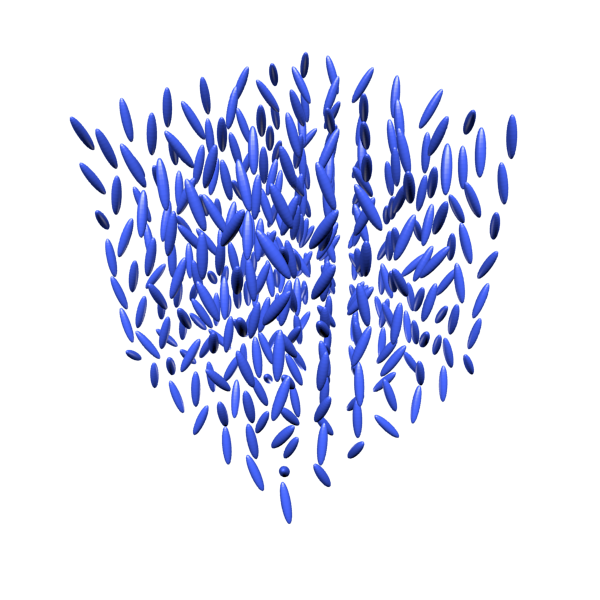
\includegraphics[height=10cm]{figures/cristaux_liquides.png} 
\end{center} 


\textbf{Résumé :} 
\vspace{0.3cm}

\textbf{Mots clefs :} cristaux liquides, nématique, Monte-Carlo.
\vspace{0.3cm}


\end{titlepage}

\newpage


\section*{Remerciements}




\tableofcontents


\newpage
\renewcommand\thepage{\arabic{page}}


\definecolor{linkcolor}{rgb}{0,0,1}

%%%%%%%%%%%%%%%%%%%%%%%%%%%%%%%%%%%%%%%%%%%%%%%%%%%%%%%%%%%%%%%%%%%%%%%%%%%%%%%%%%%%%%%%
%%%%%%%%%%%%%%%%%%%%%%%%%%%%%%%%%%%%%%%%%%%%%%%%%%%%%%%%%%%%%%%%%%%%%%%%%%%%%%%%%%%%%%%%
\section*{Introduction}
%%%%%%%%%%%%%%%%%%%%%%%%%%%%%%%%%%%%%%%%%%%%%%%%%%%%%%%%%%%%%%%%%%%%%%%%%%%%%%%%%%%%%%%%
%%%%%%%%%%%%%%%%%%%%%%%%%%%%%%%%%%%%%%%%%%%%%%%%%%%%%%%%%%%%%%%%%%%%%%%%%%%%%%%%%%%%%%%%
\addcontentsline{toc}{section}{Introduction}
Le domaine des cristaux liquides a subi une importante expansion durant tout le 20\up{ème} siècle et est encore aujourd'hui un domaine actif de la recherche en physique. L'intérêt pour ces milieux intermédiaires entre cristaux et liquides provient, entre autres, de leurs applications industrielles en matière d'afficheurs (Figure \ref{lcd_photo}).

\begin{figure}[h]
    \centering	    
	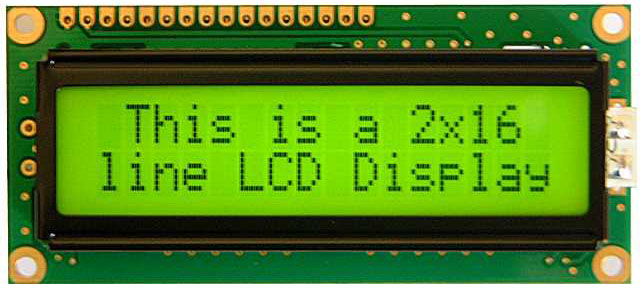
\includegraphics[height=3cm]{figures/lcd.jpg}
    \caption{Un écran à cristaux liquides}
    	\label{lcd_photo} 
\end{figure}

Le nom "cristal liquide" désigne les molécules ou mélange de molécules possédant une mésophase, c'est à dire une phase partiellement structurée, intermédiaire entre les phases liquide et cristalline. Dans ce rapport, on s'intéressera au cas particulier de la phase nématique qui emprunte aux liquides l'invariance par translation, mais brise partiellement la symétrie par rotation. Dans cette phase, les molécules s'organisent en effet pour avoir une orientation identique en moyenne (Figure \ref{nematic_phase}).

\begin{figure}[h]
    \center
    \begin{tikzpicture}[radius=0.1]
	\draw [->, >=stealth] (-1,2) -- (7.5,2) node[right]{T};
	\draw (3.35,1.9) -- (3.35,2.1) node[above]{$T^\star$};
	\draw [dashed] (3.35,2) -- (3.35,-1);

	\pgfmathsetseed{100}
	\pgfmathsetmacro{\xi}{0};
	\pgfmathsetmacro{\yi}{0};
	\foreach \i in {0,...,3}{
		\foreach \j in {0,...,2}{
			\pgfmathsetmacro{\x}{\xi+\i*0.6+0.04*rand};
			\pgfmathsetmacro{\y}{\yi+\j*0.7+0.1*rand};
			\pgfmathsetmacro{\angle}{rand*15};
			\drawZnema{\x}{\y}{\angle};
		}
	}
	\foreach \i in {0,...,3}{
		\foreach \j in {0,...,1}{
			\pgfmathsetmacro{\x}{\xi+0.3+\i*0.6+0.04*rand};
			\pgfmathsetmacro{\y}{\yi+0.35+\j*0.7+0.1*rand};
			\pgfmathsetmacro{\angle}{rand*15};
			\drawZnema{\x}{\y}{\angle};
		}
	}
	\draw [->,>=stealth] (0.5,-0.5) -- (1.5,-0.5);

	\pgfmathsetseed{79}
	\pgfmathsetmacro{\xi}{4.5};
	\pgfmathsetmacro{\yi}{0};
	\foreach \i in {0,...,3}{
		\foreach \j in {0,...,2}{
			\pgfmathsetmacro{\x}{\xi+\i*0.6+0.04*rand};
			\pgfmathsetmacro{\y}{\yi+\j*0.7+0.1*rand};
			\pgfmathsetmacro{\angle}{rand*180};
			\drawZnema{\x}{\y}{\angle};
		}
	}
	\foreach \i in {0,...,3}{
		\foreach \j in {0,...,1}{
			\pgfmathsetmacro{\x}{\xi+0.3+\i*0.6+0.04*rand};
			\pgfmathsetmacro{\y}{\yi+0.35+\j*0.7+0.1*rand};
			\pgfmathsetmacro{\angle}{rand*180};
			\drawZnema{\x}{\y}{\angle};
		}
	}


	\draw (1,-0.9) node[below]{\small phase nématique};
	\draw (5.75,-0.9) node[below]{\small phase isotrope};
\end{tikzpicture}

    \caption{Les cristaux liquides peuvent être représentés par un ensemble d'ellipsoïdes allongés dans une direction.
    Malgré les positions aléatoires des molécules, il existe un comportement collectif orientationnel : les molécules ont tendance à s'orienter, en moyenne, dans la même direction. }
    \label{nematic_phase}
\end{figure}

L'objectif de ce projet a été d'étudier, par des méthodes numériques, la transition de phase nématique-isotrope. Ce rapport présente dans un premier temps la transition de phase en question puis le modèle ainsi que les outils numériques utilisés. Les résultats obtenus sur la transition de phase observée sont ensuite détaillés. On étudiera, dans une quatrième partie, l'influence d'un champ électrique sur cette transition. Enfin, une dernière partie étudiera la transition de Fréedericksz, utilisée dans les afficheurs LCD, que l'on peut aussi observer avec notre modèle numérique.

\newpage
%%%%%%%%%%%%%%%%%%%%%%%%%%%%%%%%%%%%%%%%%%%%%%%%%%%%%%%%%%%%%%%%%%%%%%%%%%%%%%%%%%%%%%%%
%%%%%%%%%%%%%%%%%%%%%%%%%%%%%%%%%%%%%%%%%%%%%%%%%%%%%%%%%%%%%%%%%%%%%%%%%%%%%%%%%%%%%%%%
\section{Théorie de la transition nématique-isotrope}
%%%%%%%%%%%%%%%%%%%%%%%%%%%%%%%%%%%%%%%%%%%%%%%%%%%%%%%%%%%%%%%%%%%%%%%%%%%%%%%%%%%%%%%%
%%%%%%%%%%%%%%%%%%%%%%%%%%%%%%%%%%%%%%%%%%%%%%%%%%%%%%%%%%%%%%%%%%%%%%%%%%%%%%%%%%%%%%%%
\subsection{La phase nématique}
Comme expliqué dans l'introduction, les molécules en phase nématique ont tendance à avoir une orientation commune en moyenne. L'ordre est cependant purement orientationnel puisqu'elles occupent des positions aléatoires dans l'espace. Il est possible d’étudier théoriquement ces phases en définissant le directeur $\bm{n}$, comme le vecteur unitaire donnant la direction moyenne des molécules dans un volume mésoscopique. On peut noter que $\bm{n}$ et $-\bm{n}$ sont équivalents puisque rien ne change en retournant les molécules à l'envers.
\medskip

Pour décrire le degré d'alignement moléculaire dans la phase nématique, on peut considérer chaque molécule comme un bâtonnet rigide et définir le vecteur $\bm{v}$ parallèle au bâtonnet. Ce vecteur peut être repéré à l'aide des coordonnées sphériques $\theta$ et $\phi$ :
\begin{equation}
\bm{a} =
\begin{pmatrix}
 \sin \theta \cos \phi \\
 \sin \theta \sin \phi \\
 \cos \theta 
 \end{pmatrix} 
\end{equation}
Le degré d'alignement moléculaire peut donc être décrit par la densité de probabilité $f(\theta,\phi)d\Omega$ de trouver la molécule dans un angle solide $d\Omega = d\theta\, \sin \theta d\phi$ autour de la direction $(\theta,\phi)$. Si on choisit d'orienter la troisième coordonnée selon le directeur $\bm{n}$, cette fonction ne dépend pas de $\phi$ par symétrie. De plus, elle respecte $f(\theta) = f(\pi - \theta)$ puisque les molécules ont la même probabilité de pointer dans une direction ou dans celle opposée. La forme générique de cette fonction est présentée en Figure \ref{distrib}.

\begin{figure}[h]
    \centering	    
	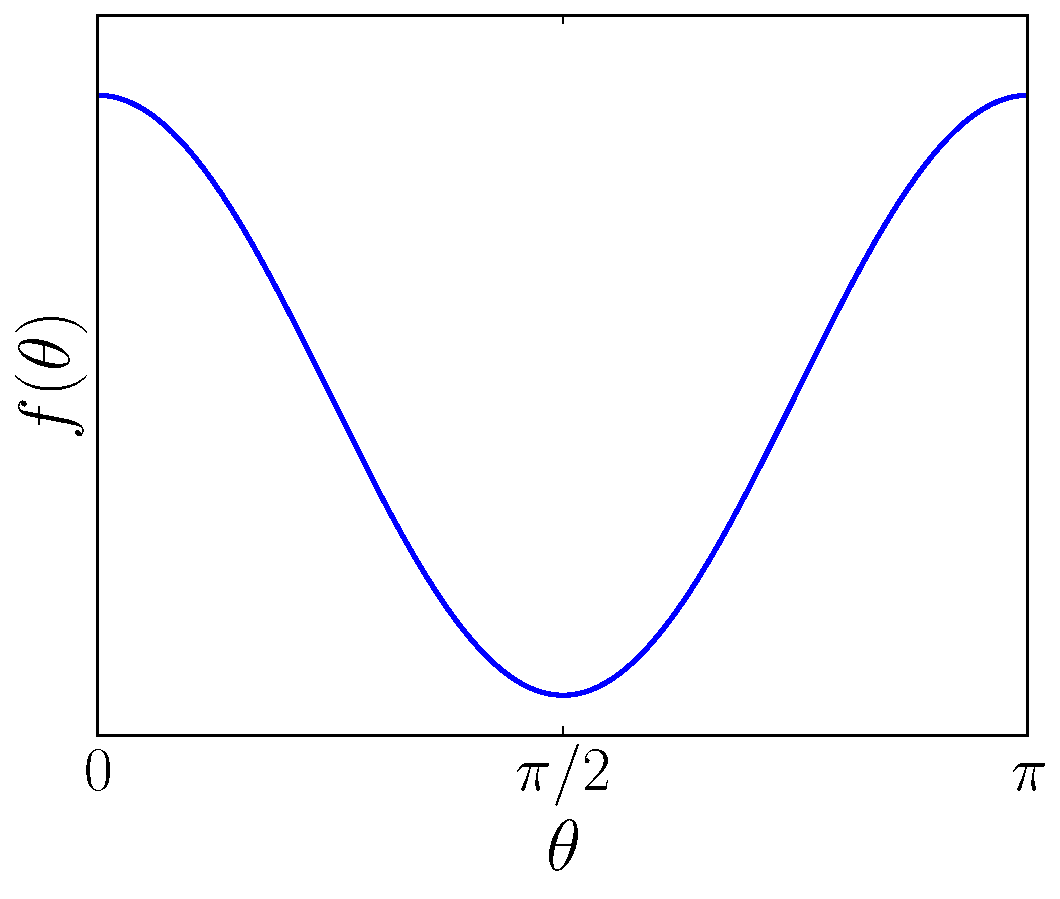
\includegraphics[scale=0.4]{figures/distrib.pdf}
    \caption{Densité de probabilité $f(\theta)$}
    	\label{distrib} 
\end{figure}

\subsection{Le paramètre d'ordre}
On essaie maintenant de construire un paramètre qui décrit l'orientation moyenne selon $\bm{n}$ et qui tend vers 0 dans la phase isotrope. Le vecteur $\langle \bm{a} \rangle $ ne convient pas car il est nul par symétrie. Une meilleure idée est d'utiliser le tenseur $\underline{\underline{S}}$ définie par :
\begin{equation}
S_{i,j} = \langle a_i a_j \rangle -\frac{1}{3} \delta_{i,j}
\label{tenseur}
\end{equation}
où $\delta_{i,j}$ est le symbole de Kronecker. Ce tenseur est non nul dans la phase nématique et s'annule bien dans la phase isotrope puisqu'on a alors $\langle  a_i a_j \rangle  = \frac{1}{3} \delta_{i,j}$. Ce tenseur est de plus symétrique et donc diagonalisable. Enfin, sa trace est nulle par construction et deux de ses valeurs propres doivent être égales par symétrie par rapport au directeur $\bm{n}$. Il se diagonalise donc dans une base $(\bm{l}, \bm{m}, \bm{n})$ sous la forme :

\begin{equation}
\underline{\underline{S}} = S
\begin{pmatrix}
 -\dfrac{1}{3} & 0  & 0\\
 0 & -\dfrac{1}{3} &0 \\
 0 &0 & \dfrac{2}{3}
 \end{pmatrix} 
 \label{matriceform}
\end{equation}
où $S$ est une amplitude. Il est possible d'obtenir l'expression de $S$ en remarquant que, d'après \ref{matriceform} :
\begin{equation*}
 \bm{n} \cdot \underline{\underline{S}} \bm{n} = 2S/3
\end{equation*} 
et que d'après l'équation \ref{tenseur} :
\begin{align*}
 \bm{n} \cdot \underline{\underline{S}} \bm{n} & = n_i\left(\langle a_i a_j \rangle-\frac{1}{3} \delta_{i,j} \right )n_j\\ 
 & = \langle n_ia_in_ja_j \rangle -\frac{1}{3}\\
 & = \langle (\bm{a}\cdot \bm{n})^2 \rangle - \frac{1}{3}
\end{align*}
de sorte que l'on ait :
\begin{equation}
S = \frac{3 \langle (\bm{a}\cdot \bm{n})^2\rangle -1}{2} = \frac{3 \langle \cos^2 \theta \rangle -1}{2}
\end{equation}

Le scalaire $S$ mesure donc le degré d'alignement selon le directeur. Il est égal à 1 lorsque toutes les molécules sont alignées selon $\bm{n}$ et il est nul dans la phase isotrope où les directions des molécules sont purement aléatoires. Il s'agit donc d'un bon choix de paramètre d'ordre pour suivre l'évolution de la transition nématique isotrope.
\newpage
%%%%%%%%%%%%%%%%%%%%%%%%%%%%%%%%%%%%%%%%%%%%%%%%%%%%%%%%%%%%%%%%%%%%%%%%%%%%%%%%%%%%%%%%
%%%%%%%%%%%%%%%%%%%%%%%%%%%%%%%%%%%%%%%%%%%%%%%%%%%%%%%%%%%%%%%%%%%%%%%%%%%%%%%%%%%%%%%%
\section{Méthodes numériques}
%%%%%%%%%%%%%%%%%%%%%%%%%%%%%%%%%%%%%%%%%%%%%%%%%%%%%%%%%%%%%%%%%%%%%%%%%%%%%%%%%%%%%%%%
%%%%%%%%%%%%%%%%%%%%%%%%%%%%%%%%%%%%%%%%%%%%%%%%%%%%%%%%%%%%%%%%%%%%%%%%%%%%%%%%%%%%%%%%
Dans cette partie, on présente le modèle de Lebwohl-Lasher utilisé ainsi que les différentes optimisations implémentés en plus de l'algorithme Monte-Carlo qui gouverne son évolution.

\subsection{Modèle de Lebwohl-Lasher}
\label{lebwohlpart}
Le modèle de Lebwohl-Lasher \cite{model} est en quelque sorte l'analogue pour la transition nématique-isotrope du modèle d'Ising. Comme pour ce dernier, il permet d'obtenir des résultats très satisfaisants malgré sa simplicité.\medskip

\begin{figure}[h]
    \center
    \begin{tikzpicture}

    \pgfmathsetseed{1}
    

    \foreach \i in {0,...,5}{
        \pgfmathsetmacro{\x}{\i*0.7};
        \draw (\x,0) -- (\x,0.7*5);
        \draw (0,\x) -- (0.7*5,\x);
    }

    \foreach \i in {0,...,5}{
    \pgfmathsetmacro{\x}{\i*0.7};
        \foreach \j in {0,1,5}{
            
            \pgfmathsetmacro{\y}{\j*0.7};
            \pgfmathsetmacro{\angle}{rand*60};
            \pgfmathsetmacro{\size}{0.3};
            \drawNema{\x}{\y}{\angle}{\size};
        }
    }

    \foreach \j in {4,2,3}{
        \pgfmathsetmacro{\y}{\j*0.7};
        \foreach \i in {0,4,5}{
            \pgfmathsetmacro{\x}{\i*0.7};
            \pgfmathsetmacro{\angle}{rand*60};
            \pgfmathsetmacro{\size}{0.3};
            \drawNema{\x}{\y}{\angle}{\size};
        }
    }


    \pgfmathsetmacro{\xc}{2*0.7};
    \pgfmathsetmacro{\yc}{3*0.7};
    \pgfmathsetmacro{\anglec}{rand*60};
    \pgfmathsetmacro{\sizec}{0.3};

    \pgfmathsetmacro{\xul}{1*0.7};
    \pgfmathsetmacro{\yul}{4*0.7};
    \pgfmathsetmacro{\angleul}{rand*60};
    \pgfmathsetmacro{\sizeul}{0.3};

    \pgfmathsetmacro{\xum}{2*0.7};
    \pgfmathsetmacro{\yum}{4*0.7};
    \pgfmathsetmacro{\angleum}{rand*60};
    \pgfmathsetmacro{\sizeum}{0.3};

    \pgfmathsetmacro{\xur}{3*0.7};
    \pgfmathsetmacro{\yur}{4*0.7};
    \pgfmathsetmacro{\angleur}{rand*60};
    \pgfmathsetmacro{\sizeur}{0.3};

    \pgfmathsetmacro{\xmr}{1*0.7};
    \pgfmathsetmacro{\ymr}{3*0.7};
    \pgfmathsetmacro{\anglemr}{rand*60};
    \pgfmathsetmacro{\sizemr}{0.3};

    \pgfmathsetmacro{\xml}{3*0.7};
    \pgfmathsetmacro{\yml}{3*0.7};
    \pgfmathsetmacro{\angleml}{rand*60};
    \pgfmathsetmacro{\sizeml}{0.3};

    \pgfmathsetmacro{\xdl}{1*0.7};
    \pgfmathsetmacro{\ydl}{2*0.7};
    \pgfmathsetmacro{\angledl}{rand*60};
    \pgfmathsetmacro{\sizedl}{0.3};

    \pgfmathsetmacro{\xdr}{3*0.7};
    \pgfmathsetmacro{\ydr}{2*0.7};
    \pgfmathsetmacro{\angledr}{rand*60};
    \pgfmathsetmacro{\sizedr}{0.3};

    \pgfmathsetmacro{\xdm}{2*0.7};
    \pgfmathsetmacro{\ydm}{2*0.7};
    \pgfmathsetmacro{\angledm}{rand*60};
    \pgfmathsetmacro{\sizedm}{0.3};

            \drawNema{\xul}{\yul}{\angleul}{\sizeul};
            \drawNema{\xum}{\yum}{\angleum}{\sizeum};
            \drawNema{\xur}{\yur}{\angleur}{\sizeur};

            \drawNema{\xml}{\yml}{\angleml}{\sizeml};
            \drawNema{\xmr}{\ymr}{\anglemr}{\sizemr};

            \drawNema{\xdr}{\ydr}{\angledr}{\sizedr};
            \drawNema{\xdl}{\ydl}{\angledl}{\sizedl};
            \drawNema{\xdm}{\ydm}{\angledm}{\sizedm};

            \drawNema{\xc}{\yc}{\anglec}{\sizec};
    


\end{tikzpicture}

    \caption{Représentation à deux dimensions du modèle de Lebwohl-Lasher.}
    \label{lebwohl}
\end{figure}


Dans ce modèle, les molécules du cristal liquide sont représentées uniquement par leur direction et occupent des positions fixes sur les sites d'un réseau cubique.
Les différents sites du réseau interagissent uniquement entre plus proches voisins par l'intermédiaire d'un potentiel de la forme :
\begin{equation}
E_{i,j}^{int} = - \epsilon\ \frac{3\cos^2\theta_{i,j}-1}{2}
\label{interact}
\end{equation}
où $\epsilon$ est une constante positive et $\theta_{i,j}$ est l'angle entre deux molécules voisines. 
Cette énergie est minimale lorsque les molécules sont parfaitement alignées : si $\theta_{i,j} = 0$ alors $E_{i,j}^{int} = - \epsilon$. Et elle est maximale lorsque les molécules ont des directions orthogonales : si $\theta_{i,j}^{int} = \pi/2$ alors $E_{i,j}^{int} = \epsilon/2$.
Ces interactions auront donc tendance à favoriser les configurations où les molécules pointent toutes dans la même direction.\medskip

On comprend alors assez bien pourquoi ce système subit une transition de phase. Les deux énergies intervenant dans ce système sont celles de l'interaction entre les molécules et celle de l'agitation thermique dont les échelles sont respectivement $\epsilon$ et $k_B T$.
À haute température, l'agitation thermique prédomine et l'orientation des molécules est aléatoire. À basse température, c'est l'énergie d'interaction entre les sites qui est la plus importante et les molécules privilégient donc une direction commune.\medskip

Pour toute notre étude de la transition de phase, des conditions aux limites périodiques ont été imposées mais d'autres conditions sont également possibles. Des travaux récents \cite{confined} ont par exemple utilisé une énergie à la surface de la même forme que le potentiel d'interaction pour simuler une cellule avec un ancrage aux parois. 

%L'énergie totale du système qui découle de cette interaction s'écrit simplement comme une somme sur les paires de plus proches voisins :
%\begin{equation}
%E = - \epsilon\ \sum_{<i,j>} \frac{3\cos^2\theta_{i,j}-1}{2}
%\end{equation}

\subsection{Algorithme Monte-Carlo}

L'idée de base derrière les algorithmes de type Monte-Carlo est de remplacer le calcul d'intégrales sur l'espace des phases par des moyennes sur une marche aléatoire. L'évolution Monte-Carlo de notre système utilise l'algorithme proposé par Metropolis et al. \cite{metropolis} qui consiste à réaliser une série de mouvements aléatoires et d'accepter ces changements avec une probabilité qui dépend de la variation d'énergie.\medskip

Plus précisément, on commence par sélectionner un site du réseau. Ensuite, une nouvelle direction de la molécule est tirée aléatoirement. Si ce changement diminue l'énergie totale du système, le changement est accepté. Sinon, le changement est accepté avec une probabilité proportionnel au poids de Boltzmann de la variation d'énergie $\Delta E$ :

\begin{equation}
p = e^{-\Delta E / k_B T}
\label{boltzmannprob}
\end{equation}
Il est important de noter que cette formule n'est valable que lorsque toute les directions ont la même probabilité d'être tirées. Sinon, il faut ajouter un facteur multiplicatif correspondant au rapport des probabilités de tirer les directions de départ et d'arrivée.
\medskip

Il est possible de montrer qu'un grand nombre de répétition de ces mouvements permet d'obtenir la configuration d'équilibre du système. Des moyennes statistiques pour les quantités d'intérêt peuvent ensuite être calculées sur les micro-états générés par l'algorithme une fois l'équilibre atteint.

\subsection{Équiprobabilité des directions}
Pour chaque site du réseau, l'orientation de la molécule est stockée en tant que $\cos \theta$ et $\phi$ où $\theta$ et $\phi$ sont respectivement les angles polaires et azimutaux. Utiliser ces variables plutôt que simplement $\theta$ et $\phi$ est nécessaire à l'équiprobabilité des directions. En effet, si l'on tire au hasard un $\theta$ et un $\phi$, la probabilité d'obtenir une direction proche du pole est plus importante (Figures \ref{a} et \ref{b}). Cette anisotropie disparaît lorsque l'on tire un $\cos \theta$ et un $\phi$ comme on peut le voir sur les Figures \ref{c} et \ref{d}. Cela se comprend assez bien en se rappelant que l'élément de surface en sphérique s'écrit $d\theta\, \sin \theta d\phi = d\text{cos}\,\theta\, d\phi$.

\begin{figure}[h!]
\center
    \begin{subfigure}[b]{0.22\textwidth}
    	\center
    	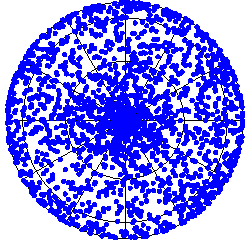
\includegraphics[height=3.5cm]{figures/dessus1.pdf}
    	\caption{Vue du dessus}
    	\label{a}
    \end{subfigure}	
	\begin{subfigure}[b]{0.22\textwidth}
    	\center
    	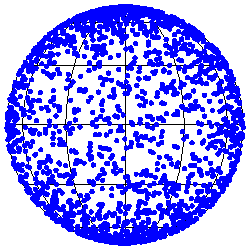
\includegraphics[height=3.5cm]{figures/side1.pdf}
    	\caption{Vue de côté}
    	\label{b}
    \end{subfigure}
		\begin{subfigure}[b]{0.05\textwidth}
		\hspace{0.1cm}
    	\center
    \end{subfigure}
    \begin{subfigure}[b]{0.22\textwidth}
    	\center
    	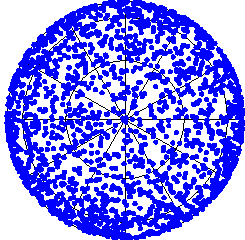
\includegraphics[height=3.5cm]{figures/dessus2.pdf}
    	\caption{Vue de dessus}
    	\label{c}
    \end{subfigure}	
    \begin{subfigure}[b]{0.22\textwidth}
    	\center
    	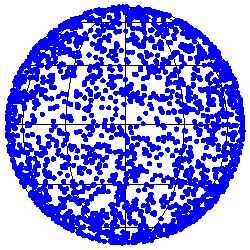
\includegraphics[height=3.5cm]{figures/side2.pdf}
    	\caption{Vue de côté}
    	\label{d}
    \end{subfigure}	
    \caption{Tirage aléatoire de 2000 directions. \ref{a}, \ref{b} : en tirant  $\theta$ et $\phi$. \ref{c}, \ref{d} : en tirant  $\cos \theta$ et $\phi$.}
    \label{equipartition}
\end{figure}
\vspace{-0.6cm}

\subsection{Ratio d'acceptation}
Le fait de choisir la nouvelle direction sur l'ensemble de la sphère unité pose certains problèmes. En effet, si l'on part de l'état fondamental où toutes les molécules sont alignées, une grande partie des mouvements tentés seront refusés car ils augmentent fortement l'énergie du système. Cet effet est plus important à basse température mais se maintient au delà de la température de transition à laquelle le ratio d'acceptation n'est encore que de $20\%$. Par conséquent, très peu de micro-états différents sont observés et les moyennes calculées ne rendent alors pas bien compte du système.
\medskip

Pour palier à ce problème il est possible de restreindre l'amplitude des changements de directions. Si les changements sont petits, le ratio d'acceptation sera grand puisque chaque mouvement ne changera que très peu l'énergie du système. Cependant, comme le système n'évolue qu'en réalisant de petits changements, le temps d'équilibrage du système sera long. Inversement, de grands changements dérangent l'équilibre local et résultent en une forte augmentation de l'énergie. Par conséquent, il est peu probable que ces changements soient accepté et du temps de calcul est gâché à créer des pas refusées.
\medskip

Finalement, il est possible d'obtenir un ratio d'acceptation de $50\%$ sur toute la durée de la simulation et ce pour n'importe quelle température. Pour cela, il suffit d'adapter l'amplitude des changements au ratio d'acceptation au fur et à mesure de la simulation. Si le ratio est inférieur à $50\%$, trop de pas sont refusés et il suffit de diminuer l'amplitude des changements pour augmenter le ratio d'acceptation. Si le ratio est supérieur à $50\%$, trop de pas sont acceptés et il suffit d'augmenter l'amplitude des changements pour diminuer le ratio d'acceptation. 
\medskip

Le choix d'un ratio d'acceptation de $50\%$ a été fait de manière arbitraire. Même si certaines recherches \cite{acceptanceratio} semblent montrer qu'un ratio d'acceptation entre $30\%$ et $50\%$ serait optimal, il s'agit encore aujourd'hui d'une question ouverte sur les algorithmes Monte-Carlo \cite{acceptanceratio1}.

\subsection{Déroulement d'une simulation} 
Les simulations reportées dans ce rapport ont toutes été réalisées sur un réseau cubique de taille $30\times 30\times 30$. Les conditions aux limites sont prises périodiques sauf dans le dernier chapitre où on considère un ancrage aux bords. Les simulations sont commencées depuis l'état fondamental où toutes les molécules sont alignées. Lorsque l'on démarre la simulation, les molécules sont bougées les unes après les autres en utilisant l'algorithme de Monte-Carlo. On nomme "cycle" une suite de $N = 30\times 30\times 30$ mouvements. Durant un cycle, toutes les molécules du réseau sont bougées exactement une fois mais dans un ordre aléatoire. Une telle procédure assure que toutes les molécules ont la même chance d'être bougée en réduisant les irrégularités dues à un tirage totalement aléatoire \cite{fabbri}. 
\medskip

Pour chaque température, au minimum 2000 cycles sont calculés pour faire évoluer le système vers la configuration d'équilibre . Même pour les températures élevées, seuls 300 cycles sont nécessaires. Par précaution, les variations de l'énergie et du paramètre d'ordre sont contrôlées pour vérifier que le système est bien à l'équilibre (Figure \ref{equilibrage}). Ensuite, jusqu'à 30000 cycles sont réalisés afin de calculer les quantités d'intérêt.

\begin{figure}[h!]
    \centering	    
	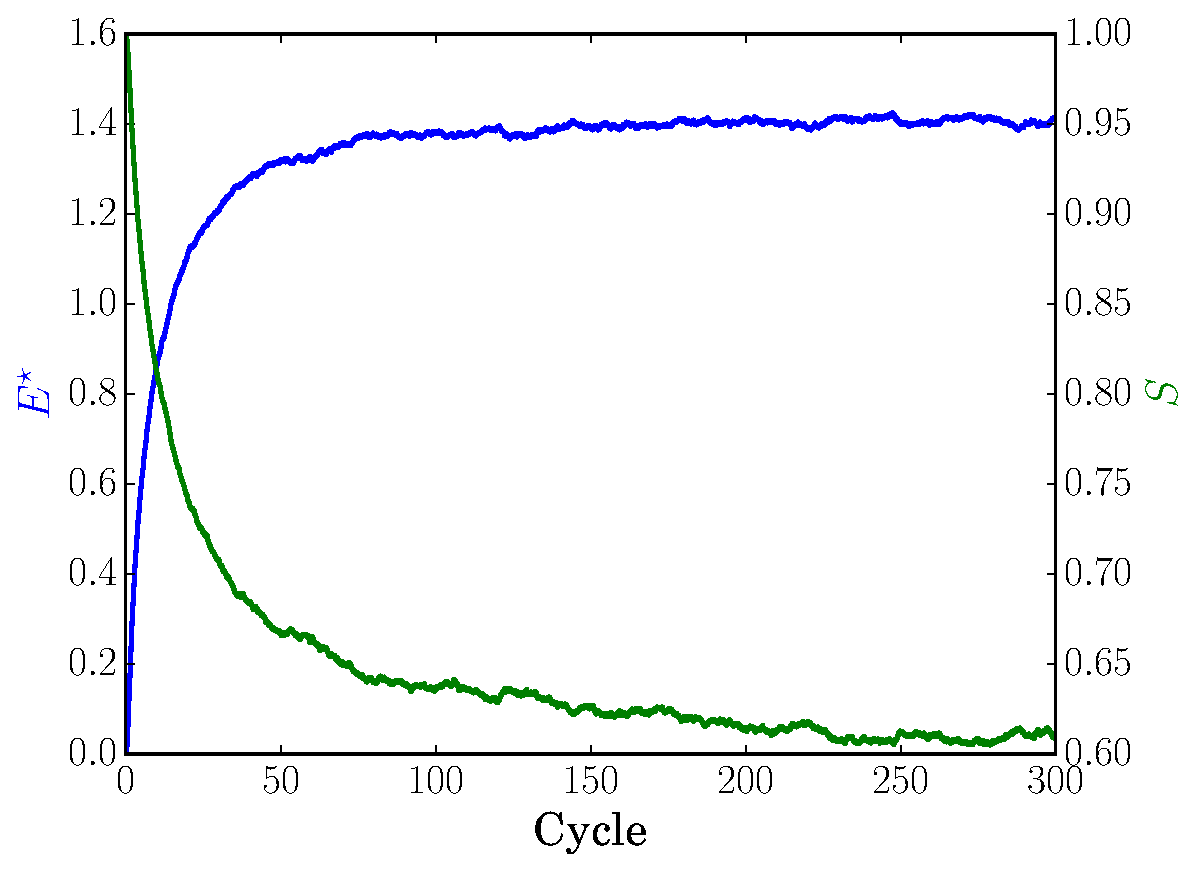
\includegraphics[scale=0.6]{figures/equilibrage.pdf}
    \caption{Observation de l'équilibrage du système à une température $T^\star = k_B T/\epsilon = 1$ en partant de l'état fondamental. L'énergie renormalisée (voir partie \ref{scale}) ainsi que le paramètre d'ordre sont représentés en fonction des cycles}
    	\label{equilibrage} 
\end{figure}


\subsection{Langage de programmation}
Une première version du code a été implémentée en \texttt{Python} et a permis d'obtenir simplement des résultats. L'existence de bibliothèque comme \texttt{Numpy} permet d'obtenir un code fonctionnant de manière rapide et intuitive. Cependant, \texttt{Python} n'est pas adapté à des algorithmes de type Monte-Carlo qui consistent en de longues itérations. Ainsi, une seconde version du code plus performante a été implémentée en \CC. Ce dernier tourne en moyenne 40 fois plus vite que son homologue en \texttt{Python} ce qui a permis de réaliser de plus grosses simulations. L'utilisation des ressources du Centre Blaise Pascal a également été d'une grande aide pour réaliser des simulations sur une longue durée. Les deux versions du code sont disponibles en libre accès sur la plateforme github \cite{github}.
\newpage
%%%%%%%%%%%%%%%%%%%%%%%%%%%%%%%%%%%%%%%%%%%%%%%%%%%%%%%%%%%%%%%%%%%%%%%%%%%%%%%%%%%%%%%%
%%%%%%%%%%%%%%%%%%%%%%%%%%%%%%%%%%%%%%%%%%%%%%%%%%%%%%%%%%%%%%%%%%%%%%%%%%%%%%%%%%%%%%%%
\section{Transition nématique-isotrope}
%%%%%%%%%%%%%%%%%%%%%%%%%%%%%%%%%%%%%%%%%%%%%%%%%%%%%%%%%%%%%%%%%%%%%%%%%%%%%%%%%%%%%%%%
%%%%%%%%%%%%%%%%%%%%%%%%%%%%%%%%%%%%%%%%%%%%%%%%%%%%%%%%%%%%%%%%%%%%%%%%%%%%%%%%%%%%%%%%
Dans cette partie, on présente les différents résultats obtenus sur la transition de phase observée. 
%La transition de phase est introduit dans une première sous-partie. On détaillera ensuite l'étude de la température de transition qui a représenté la majeur partie du temps de travail. Enfin, une dernière partie 
\subsection{Échelle de température et d'énergie.}
\label{scale}
Dans un premier temps, on peut détailler les grandeurs importantes du modèle de Lebwohl-Lasher pour cette transition de phase.
\medskip

Bien entendu, l'échelle caractérisant les énergies est $\epsilon$, qui apparaît dans la formule \ref{interact}. Dans cette étude, toutes les quantités énergétiques ont donc été renormalisées par rapport à $\epsilon$ et $N$, qui est le nombre de site dans la lattice. De plus, les échelles énergétiques ont été décalées de sorte que l'état fondamental soit d'énergie nulle. Pour résumer, les énergies représentées dans ce rapport correspondent à l'énergie moyenne stockée dans un site et écrit en unité de $\epsilon$ : $E^\star=E/N\epsilon$.
\medskip

Ensuite, le seul endroit où intervient la température dans ce modèle est dans la probabilité d'accepter un pas \ref{boltzmannprob}. Ainsi, on peut définir la température réduite $T^\star = k_B T /\epsilon$ qui est celle importante pour la transition.

\subsection{Observation de la transition}
\begin{figure}[h!]
\center
    \begin{subfigure}[b]{0.30\textwidth}
    	\center
    	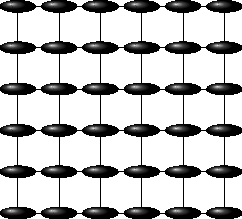
\includegraphics[scale=1]{figures/00.pdf}
    	\caption{$T^\star =0.05$}
    	\label{fonda}
    \end{subfigure}	
	\begin{subfigure}[b]{0.30\textwidth}
    	\center
    	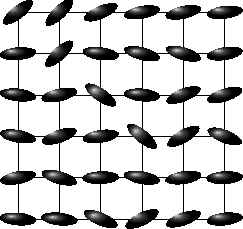
\includegraphics[scale=1]{figures/09.pdf}
    	\caption{$T^\star =0.9$}
    	\label{09}
    \end{subfigure}
    \begin{subfigure}[b]{0.30\textwidth}
    	\center
    	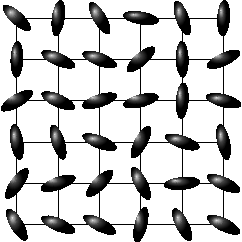
\includegraphics[scale=1]{figures/15.pdf}
    	\caption{$T^\star =1.5$}
    	\label{15}
    \end{subfigure}	
    \caption{Une partie du réseau pour trois températures différentes. Seul l'angle $\theta$ est utilisé pour cette représentation. }
    \label{lattice}
\end{figure}

Une première méthode pour observer la transition de phase est d'afficher directement l'état du réseau à la fin de l'équilibrage (Figure \ref{lattice}). À température proche de 0 (Figure \ref{fonda}), l'état d'équilibre est très proche de l'état fondamental et toutes molécules sont presque alignées. Lorsque l'on augmente la température jusqu'à $T^\star = 0.9$ (Figure \ref{09}), l'agitation thermique joue un rôle plus important et l'alignement n'est plus parfait. On peut cependant clairement observer une orientation commune en moyenne des molécules. Pour des températures plus élevées (Figure \ref{15}), l'agitation thermique prédomine et l'orientation des molécules est complètement aléatoire.
On passe donc d'un état ordonné à un état aléatoire. La transition entre ces deux états semble s'effectuer à une température entre $T^\star = 0.9$ et $T^\star = 1.5$. 
\medskip

Cette idée de la température de transition obtenue par visualisation directe donne la gamme de température sur laquelle on souhaite calculer les quantités d'intérêts que sont l'énergie $E^\star$ et le paramètre d'ordre $S$. La Figure \ref{global} représente l'énergie et le paramètre d'ordre sur une large gamme de température. Pour cette étude, on a moyenné ces quantités sur 5000 cycles. La résolution en température est de l'ordre du centième d'unité (200 températures réalisées).
\medskip

Sur cette figure, on observe que la transition de phase se fait à une température $T^\star$ proche de 1.12. On le voit grâce à la rupture de pente apparaissant dans l'énergie qui est caractéristique des transitions du premier ordre. Il est également possible d'observer la transition à l'aide du paramètre d'ordre $S$ qui s'annule à la transition.

\begin{figure}[h!]
    \centering	    
	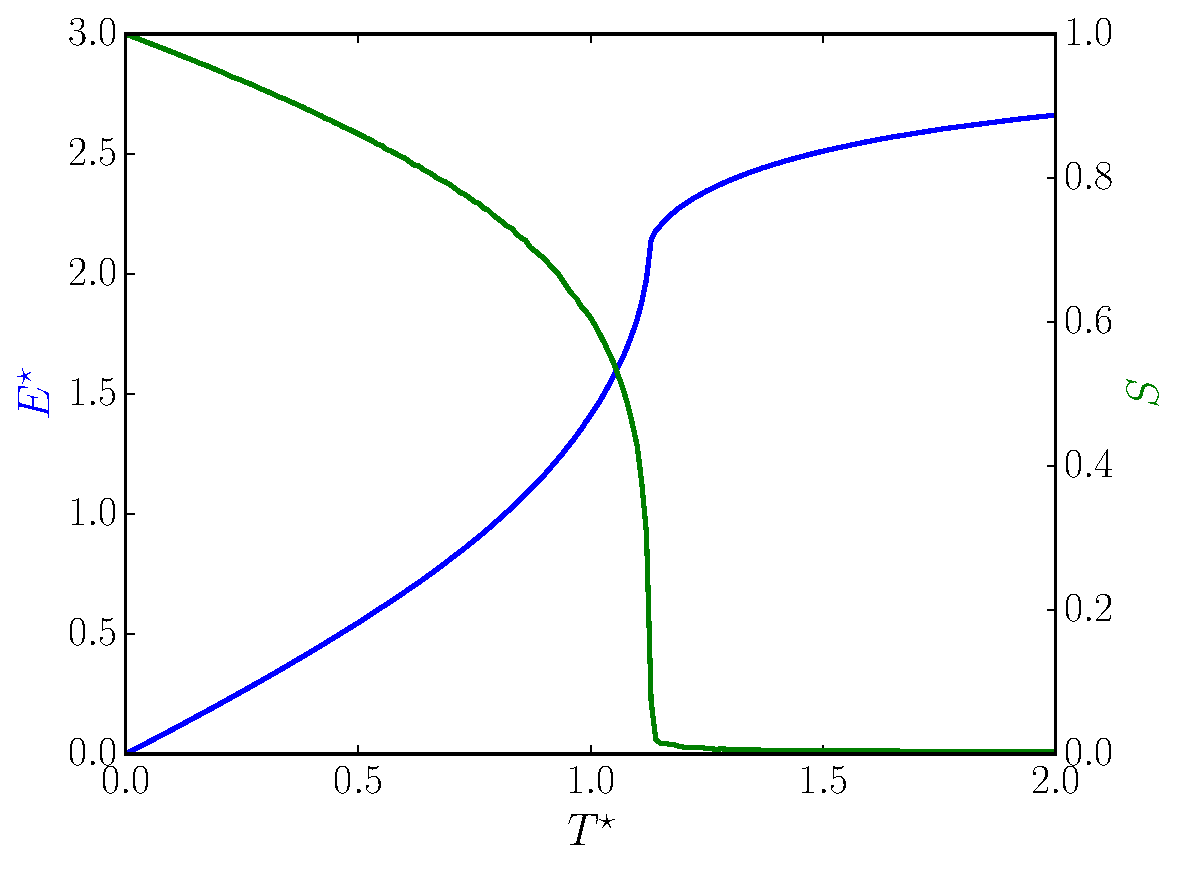
\includegraphics[scale=0.6]{figures/global.pdf}
    \caption{Énergie et paramètre d'ordre en fonction de la température.}
    	\label{global} 
\end{figure}


\subsection{Température de transition}
\label{temptrans}
Afin de déterminer plus précisément la température de transition, d'autres simulations ont été réalisées. La gamme de température observée est beaucoup plus restreinte de manière à avoir une meilleure résolution en température. De plus, les simulations ont été reproduites une trentaine de fois. Les résultats ont donc été moyennés sur les différentes simulations pour réduire la possibilité d'une réalisation particulière donnant une mauvaise température de transition.  Par exemple, le système peut évoluer vers des configurations bloquées desquels il serait difficile de sortir ce qui pourrait fausser les valeurs des observables mesurées.   

\begin{figure}[h!]
    \centering	    
	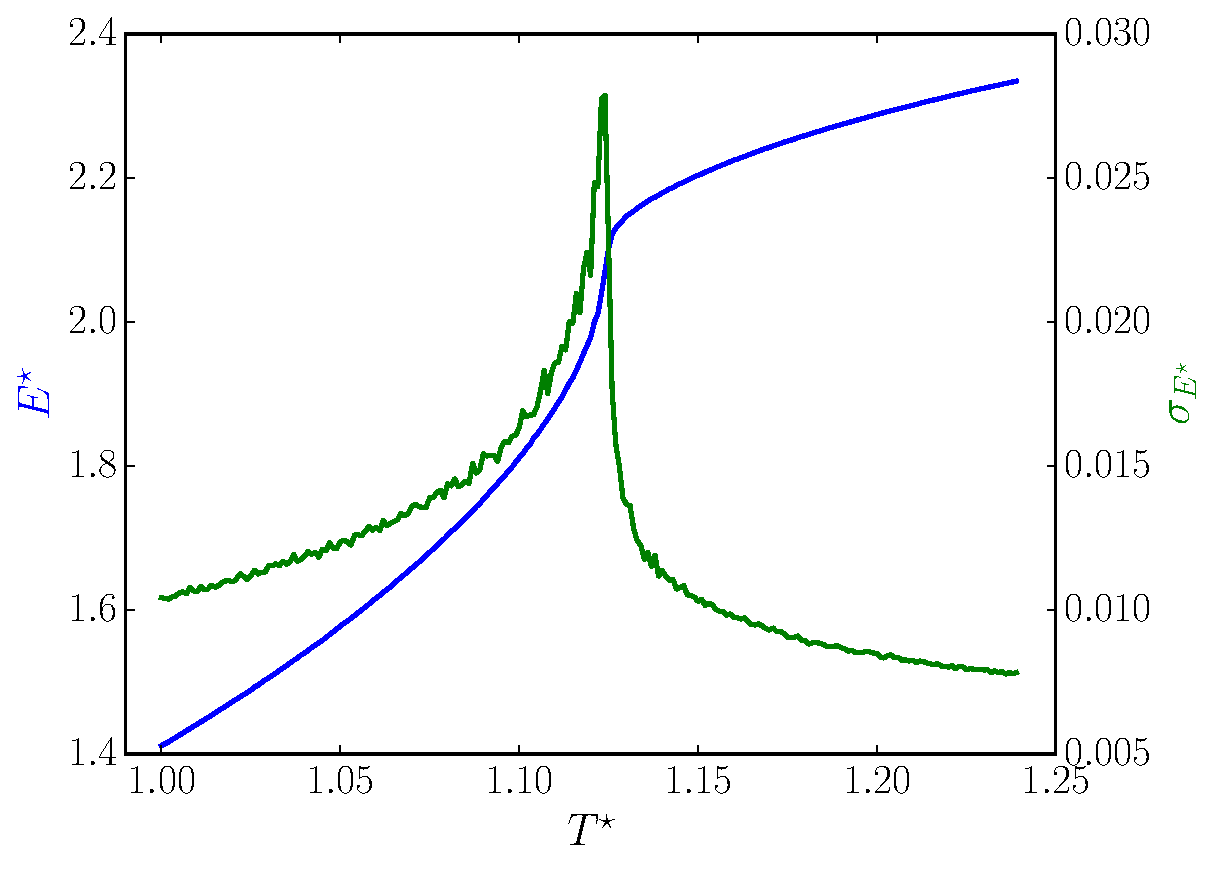
\includegraphics[scale=0.6]{figures/local_energie.pdf}
    \caption{Énergie et variance de l'énergie en fonction de la température.}
    	\label{local_energie} 
\end{figure}

Les Figures \ref{local_energie} et \ref{local_order} sont le résultat de ces moyennes sur les réalisations. Elles représentent l'énergie, le paramètre d'ordre ainsi que leurs variances en fonction de la température. Ces quantités sont moyennés sur 5000 cycles pour chacune des 240 températures réalisées.
\medskip

Commençons par étudier la figure \ref{local_energie}. Comme sur la Figure \ref{global}, on observe une rupture de pente très marquée pour une température proche de 1.12. Plus précisément, la rupture de pente apparaît pour la température $T^\star = 1.1232 \pm 0.0005$. Cette valeur correspond parfaitement aux valeurs trouvées dans la littérature \cite{fabbri,wfo, parallel, badass}. Il est également possible de déterminer la température de transition à l'aide de la variance de l'énergie en fonction de la température. Cette variance correspond à un facteur multiplicatif près à la capacité calorifique qui est censée passer par un pic à la transition. La détermination de la température de transition par le maximum de cette variance donne le même résultat avec une incertitude très légèrement supérieure : $T^\star = 1.1232 \pm 0.0006$.

\begin{figure}[h!]
    \centering	    
	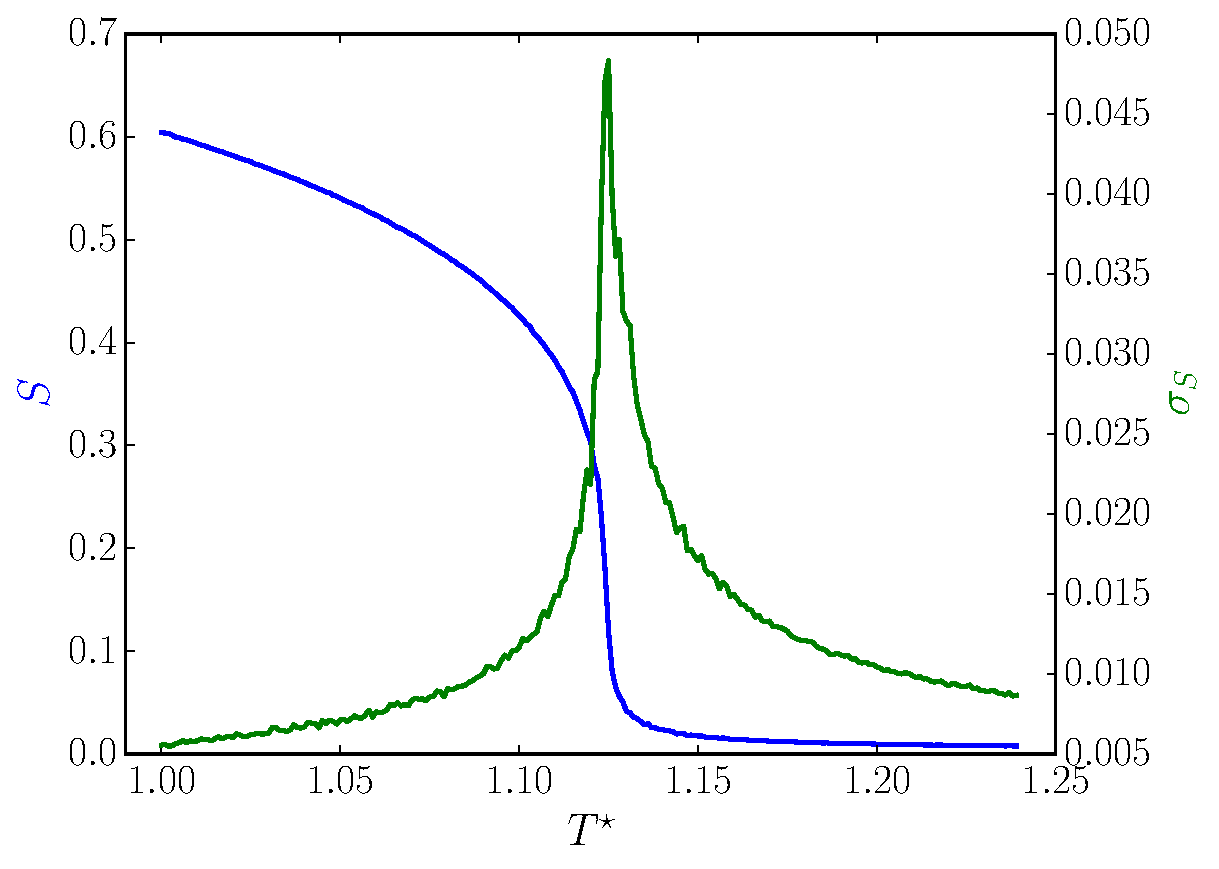
\includegraphics[scale=0.6]{figures/local_order.pdf}
    \caption{Paramètre d'ordre et variance du paramètre d'ordre en fonction de la température.}
    	\label{local_order} 
\end{figure}

Ensuite, on peut s'intéresser à l'évolution du paramètre d'ordre avec la température sur la Figure \ref{local_order}. Ce dernier chute d'une valeur de 0.4 à une valeur presque nulle après la transition. La plus grosse chute de paramètre d'ordre se fait pour la température $T^\star = 1.1231 \pm 0.0005$. Comme pour l'énergie, on peut s'intéresser à la variance du paramètre d'ordre qui correspond donc maintenant à sa susceptibilité. Cette dernière passe par un maximum à une température $T^\star = 1.123 \pm 0.001$. Cette mesure est celle pour laquelle les incertitudes sont les plus grandes des 4 réalisées.
\medskip

Sur cette figure, on observe de plus que le paramètre d'ordre ne s'annule pas directement après la température de transition. Cet effet provient de la taille finie du système et est amplifié par les moyennes sur les réalisations. Des travaux récents \cite{cluster,nonb} étudient cet effet en fonction de la taille du réseau. En extrapolant ensuite leurs résultats à un système de taille infinie ils en déduisent la température de transition de manière extrêmement précise. La température obtenue par ces méthodes est de $T^\star = 1.1232 \pm 0.0001$.

\newpage

\subsection{Histogrammes en énergie}

Une dernière méthode pour étudier la transition est de s'intéresser au histogrammes des occurrences d'une certaine énergie. Pour générer des résultats satisfaisants, il a été nécessaire de réaliser des simulations bien plus longues que les précédentes. Pour chacune des 100 températures prises entre 1.10 et 1.14, les histogrammes ont été générées sur 30 000 cycles. À titre d'information, une telle simulation prend une centaine d'heures sur les machines performantes du Centre Blaise Pascal. On présente en figure \ref{imagehisto} et \ref{histoo} les histogrammes en énergie générés à partir de ces simulations.

\begin{figure}[h!]
    \centering	    
	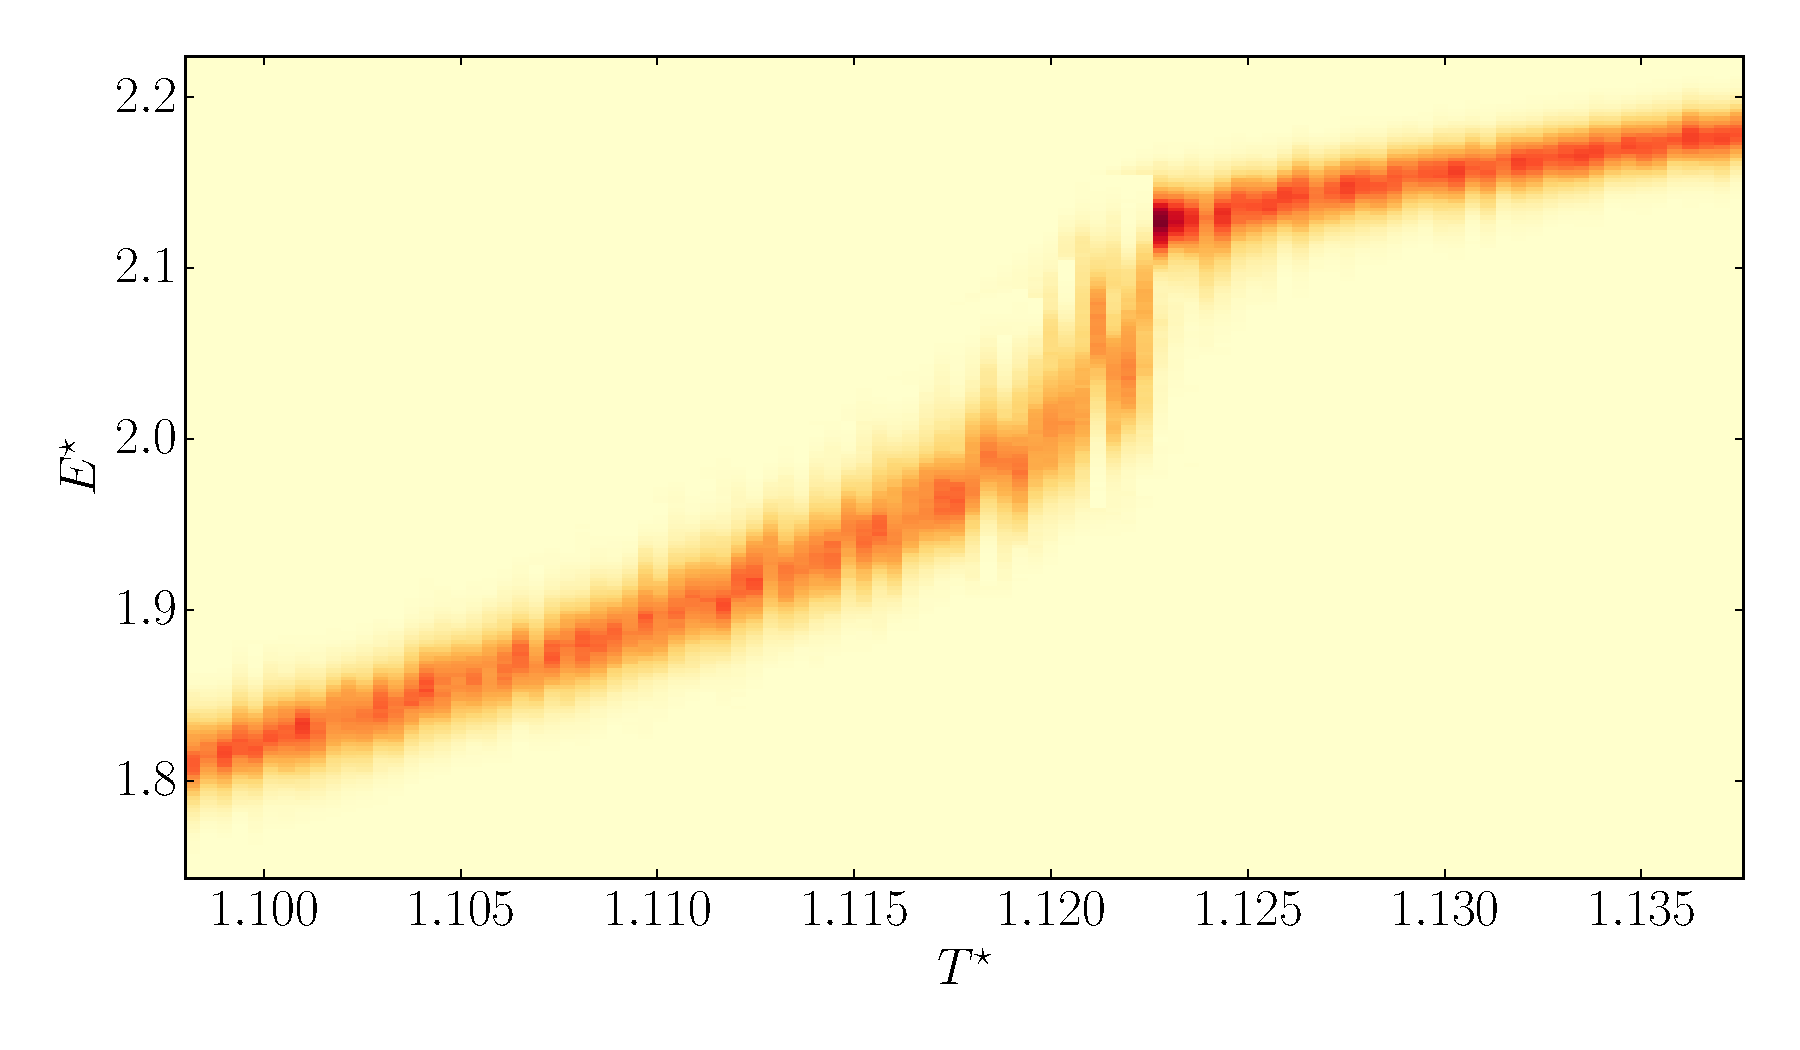
\includegraphics[scale=0.5]{figures/histo_image.pdf}
    \caption{Histogramme en énergie en fonction de la température. Le nombre d’occurrence pour chaque énergie est représentée en fausses couleurs.}
    	\label{imagehisto} 
\end{figure}
Sur la Figure \ref{imagehisto}, on peut voir les histogrammes obtenus pour chaque température. Sur cette image, on retrouve le profil observé en Figure \ref{local_energie} avec la rupture de pente des énergies. Proche de la transition, les histogrammes sont plus étendus ce qui correspond bien au pic de la variance. Enfin, on constate clairement un saut en énergie à la température 1.123. Le recouvrement entre les histogrammes avant et après cette température est pratiquement nul.
\medskip

Sur les histogrammes de la figure \ref{histoo}, on n'observe pas juste un décalage progressif des énergies avec la température mais plutôt un comportement en double pic. Pour une température juste en dessous de la transition (Figure \ref{11208}), on voit un grand pic situé à 2.03 et un plus petit à 2.11. Pour une température juste au dessus de la transition (Figure \ref{11240}), les deux pics sont toujours visibles mais l'intensité des deux pics est échangée. Ce comportement laisse supposer l'existence de deux configurations stables dans lesquelles le système passe des temps longs. Il transfère rapidement de l'une vers l'autre. On a pu vérifier en visualisant directement l'énergie en fonction des cycles que le système alterne entre ces deux états. En s'intéressant au paramètre d'ordre, on a pu de plus constater que l'état de faible énergie a un paramètre d'ordre plus élevé et correspond donc à un état ordonné contrairement au second état qui est gouverné par l'aléatoire.
\medskip

Un tel comportement en double pic est attendu pour les transitions de phase du premier ordre. Ce comportement a été également observé dans un modèle plus grossier \cite{model} dans lequel les orientations prises par les molécules sont discrètes, on peut aussi le voir de manière moins évidente dans d'autres articles \cite{fabbri}.

\begin{figure}
\center
    \begin{subfigure}[b]{0.49\textwidth}
    	\center
    	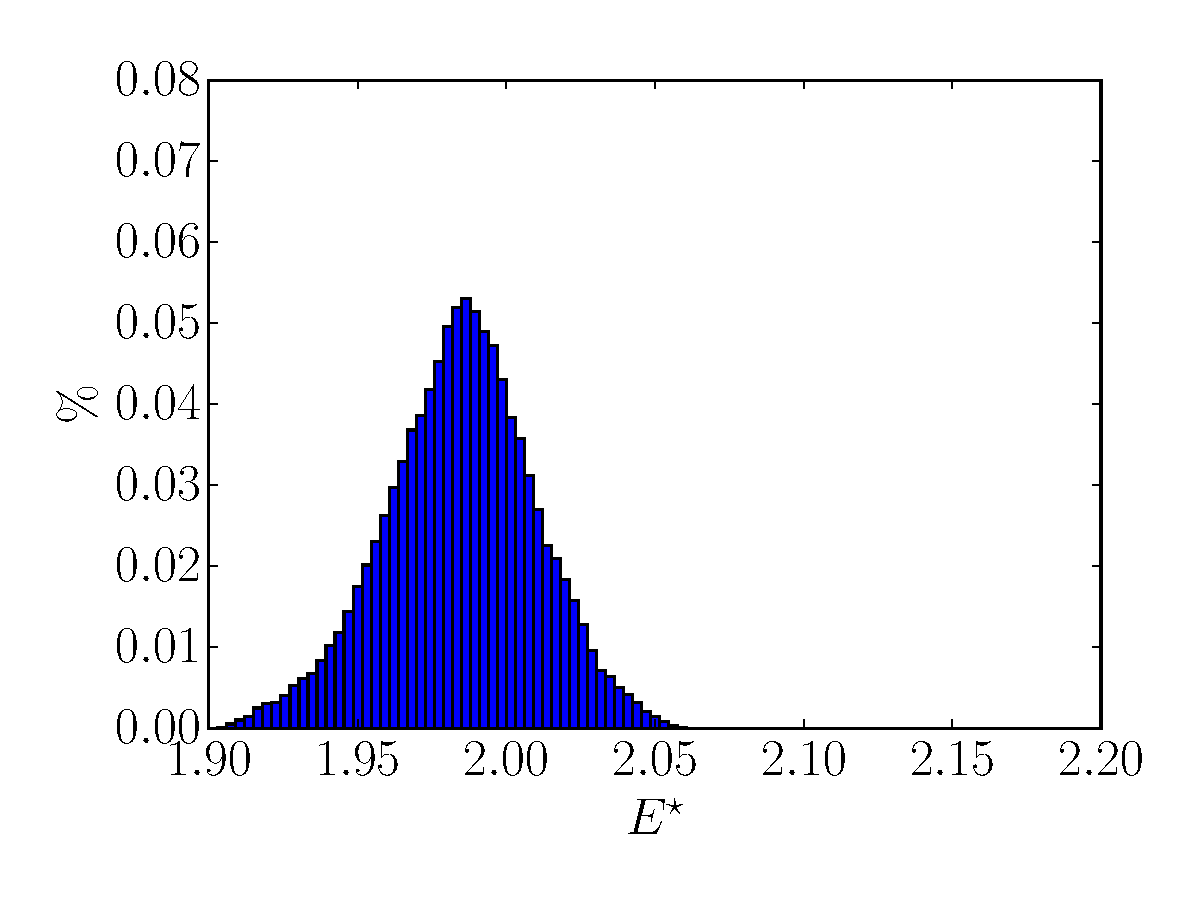
\includegraphics[scale=0.4]{figures/histo_11208.pdf}
    	\caption{$T^\star =1.1208$}
    	\label{11208}
    \end{subfigure}	
	\begin{subfigure}[b]{0.49\textwidth}
    	\center
    	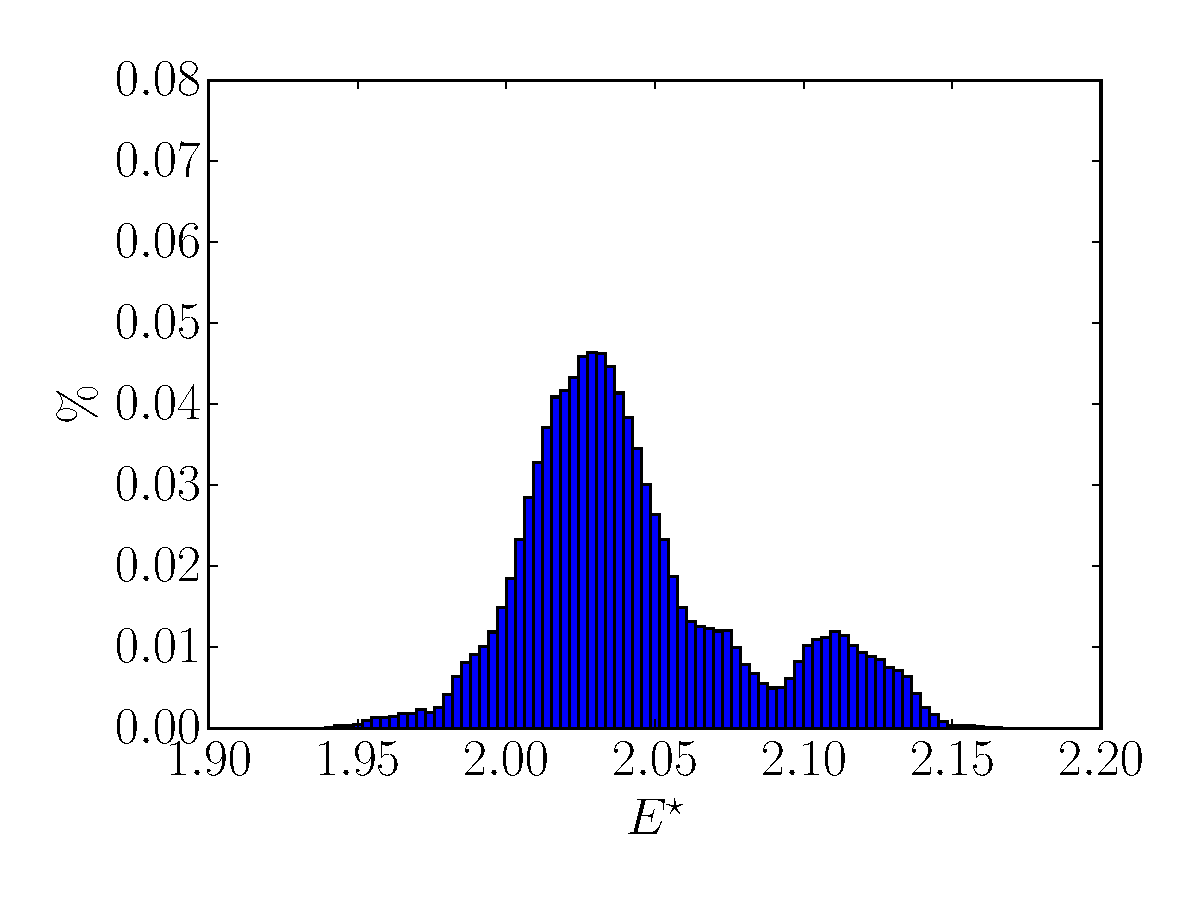
\includegraphics[scale=0.4]{figures/histo_11228.pdf}
    	\caption{$T^\star =1.1228$}
    	\label{11228}
    \end{subfigure}
    
    \begin{subfigure}[b]{0.49\textwidth}
    	\center
    	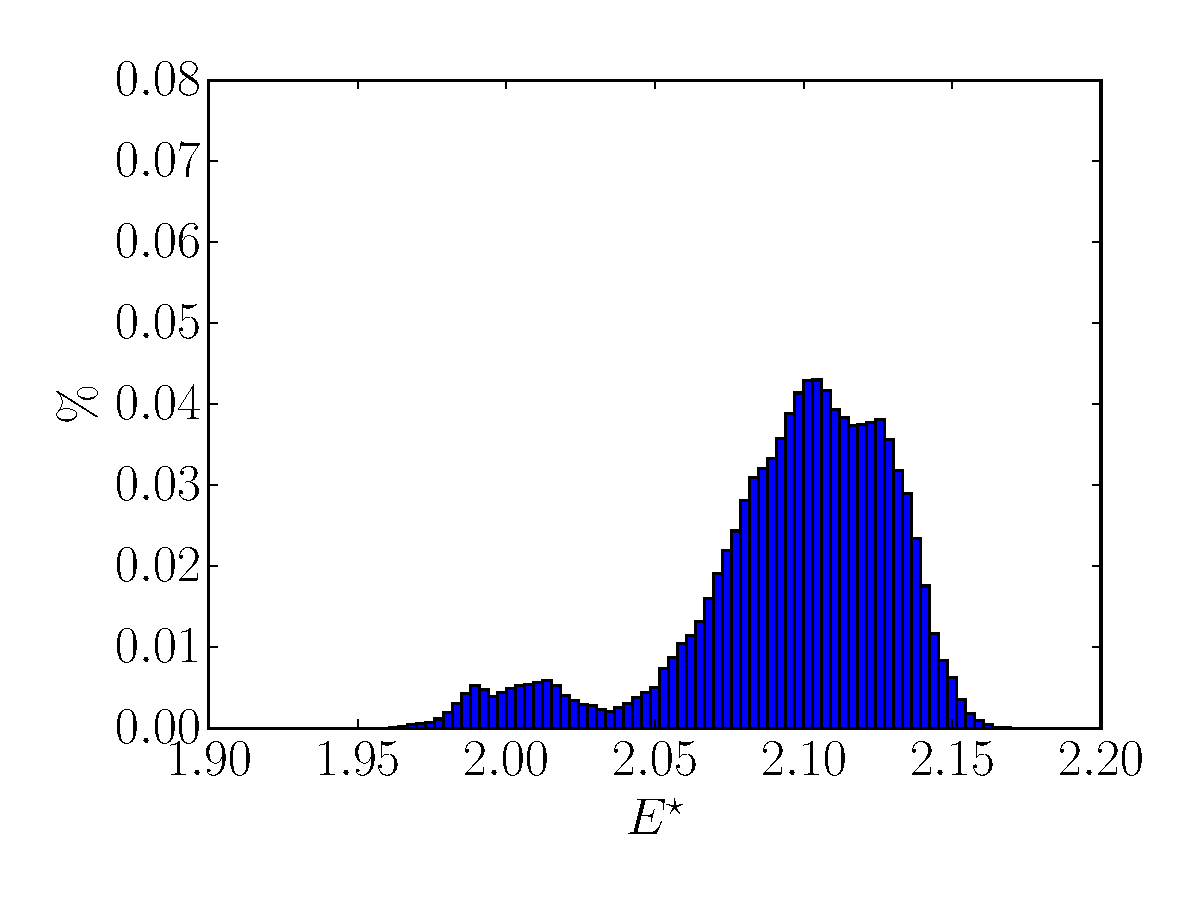
\includegraphics[scale=0.4]{figures/histo_11240.pdf}
    	\caption{$T^\star =1.1240$}
    	\label{11240}
    \end{subfigure}	
    \begin{subfigure}[b]{0.49\textwidth}
    	\center
    	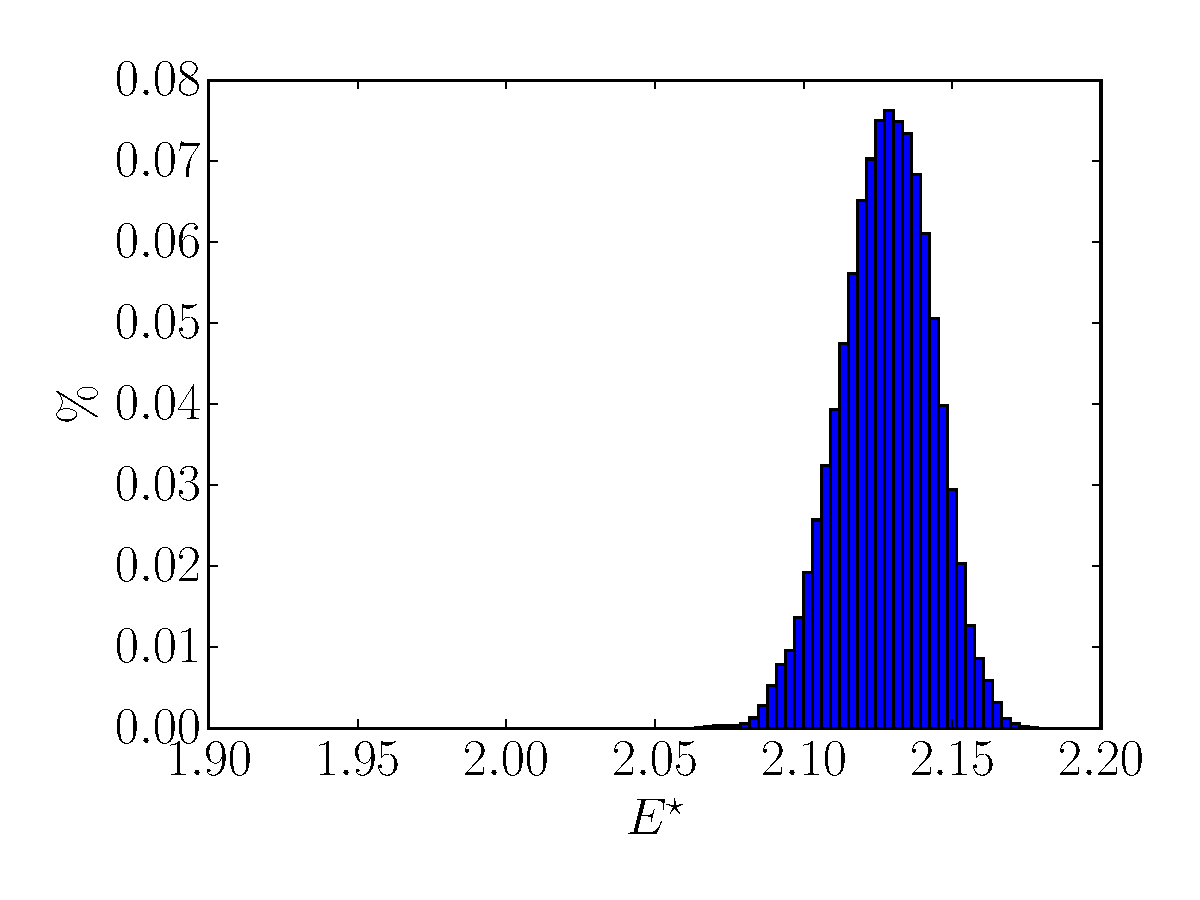
\includegraphics[scale=0.4]{figures/histo_11256.pdf}
    	\caption{$T^\star =1.1256$}
    	\label{11256}
    \end{subfigure}	
    \caption{Histogramme des énergies pour quatre températures. Pour rappel la transition a lieu à $T^\star = 1.1232$. Les deux graphes (a) et (b) sont donc avant la transition et (c) et (d) sont après.}
    \label{histoo}
\end{figure}

\newpage
%%%%%%%%%%%%%%%%%%%%%%%%%%%%%%%%%%%%%%%%%%%%%%%%%%%%%%%%%%%%%%%%%%%%%%%%%%%%%%%%%%%%%%%%
%%%%%%%%%%%%%%%%%%%%%%%%%%%%%%%%%%%%%%%%%%%%%%%%%%%%%%%%%%%%%%%%%%%%%%%%%%%%%%%%%%%%%%%%
\section{Influence d'un champ électrique}


Dans cette partie on s'intéresse à l'influence d'un champ électrique sur la transition nématique isotrope, toujours à l'aide du modèle de Lebwohl-Lasher. Comme les molécules ont tendances à s'orienter dans la direction du champ électrique, ce dernier stabilise la phase nématique. L'objectif de cette partie est donc de tracer la température de transition en fonction du champ électrique.
\subsection{Ajout au modèle de Lebwohl-Lasher}
Le champ électrique peut être incorporé au modèle décrit en partie \ref{lebwohlpart} en ajoutant en terme dans l'énergie prenant en compte le couplage entre l'orientation des molécules et le champ électrique. Ce dernier est de la même forme que le potentiel entre deux molécules \cite{entropicelectric,electric3, biolo}:
\begin{equation}
E_{i}^{el} = - \epsilon \xi U^2 \frac{3\cos^2\alpha_i-1}{2}
\label{interactfield}
\end{equation}
où $\xi$ est une constante positive, $U$ le champ électrique et $\alpha_{i}$ l'angle entre la molécule et le champ. La quantité importante dominant l'évolution en champ électrique est $U^\star = \sqrt{\xi} U$ et sera donc utilisée dans les graphes qui suivent. L'énergie totale du système qui apparaît dans l'algorithme Monte-Carlo est donc la somme des interactions entre voisins et des interactions avec le champ :
\begin{equation}
E = - \epsilon\sum_{<i,j>} \frac{3\cos^2\theta_{i,j}-1}{2} - \epsilon \xi U^2 \sum_{i}\frac{3\cos^2\alpha_i-1}{2}
\end{equation}

\subsection{Température de transition}
Avec un tel potentiel, les configurations où les molécules sont alignées avec le champ sont plus stables. Cette énergie supplémentaire vient donc stabiliser la phase nématique lorsque le champ et les molécules sont alignées. On s'attend donc à avoir une augmentation de la température de transition avec le champ électrique.

\begin{figure}[h!]
    \centering      
    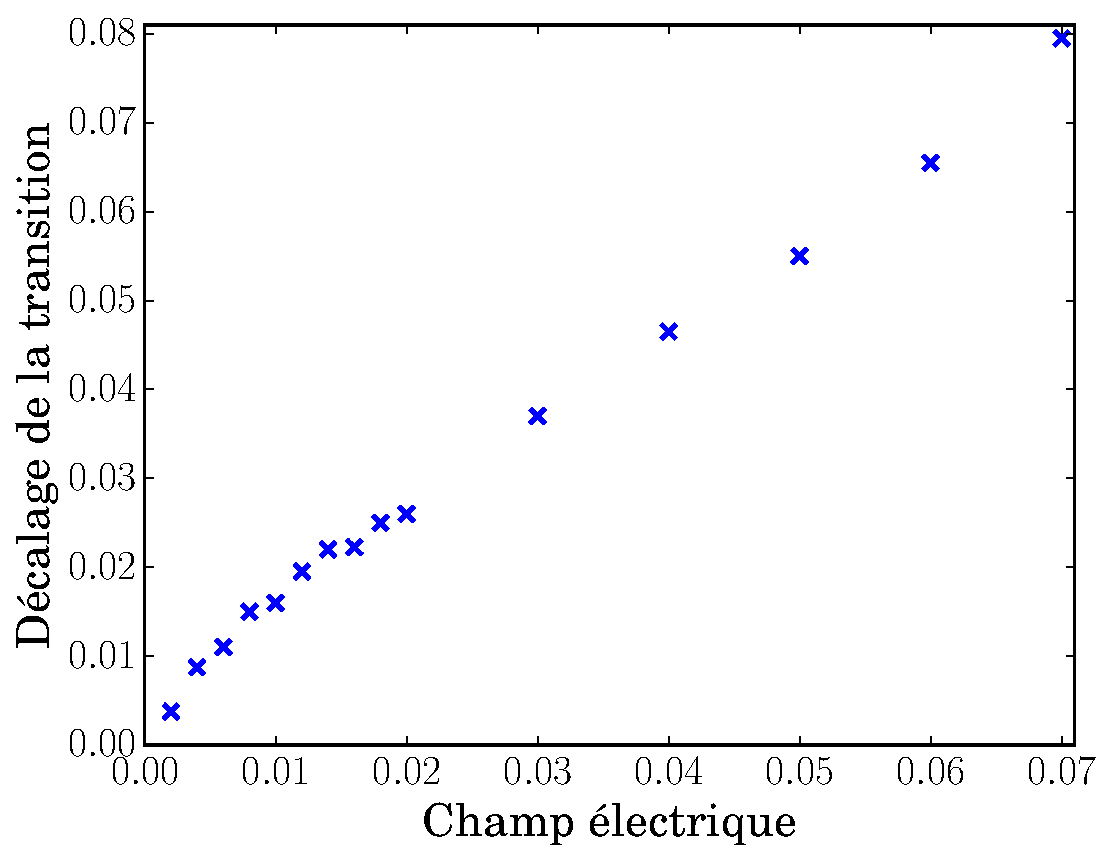
\includegraphics[scale=0.6]{figures/electricField.pdf}
    \caption{Décalage par rapport à la température de transition $T^\star$. La ligne en trait plein correspond à un ajustement linéaire des données pour les champs faibles. La ligne en tirets correspond à un ajustement quadratique des données pour les champs forts.}
        \label{electricField} 
\end{figure}

\newpage

Pour vérifier cela, il est possible de réaliser une étude similaire à celle présentée en partie \ref{temptrans} pour plusieurs champ électrique. Pour chacune des valeurs de champ souhaitées, on réalise une dizaine de simulations sur 200 températures de $T^\star = 1.00$ à $T^\star = 1.20$. Avec les résultats, on peut tracer les graphes d'énergie et de paramètre d'ordre et déterminer la température de transition pour chaque champ électrique. Le résultat de cette étude est présenté en Figure \ref{electricField}.
\medskip

Comme on peut le voir sur la figure \ref{electricField}, la température de transition de phase se comporte comme attendu: elle augmente avec le champ électrique. On peut cependant distinguer deux régimes. Pour les petites valeurs du champ (inférieur à 0.04), le décalage en température est linéaire. Il tend à devenir quadratique avec l'intensité du champ pour des valeurs plus élevées. Ces deux régimes ont été observés dans plusieurs articles de la littérature \cite{entropicelectric, field}. Enfin, on peut noter que le régime linéaire concorde avec les prévisions d'un calcul à la Landau \cite{landau}.

\subsection{Existence d'un point critique}
Cette augmentation de la température de transition avec le champ électrique a également été observé expérimentalement \cite{mfieldExperiment,efieldExperiment,efieldExperiment2}. Ces études ont de plus montré que cette transition finit en point critique pour les champs forts \cite{efieldExperiment}. L'existence d'un point critique pour cette transition apparaît également dans nos simulations. On constate en effet un adoucissement de la transition lorsque le champ électrique augmente. Cet effet est visible en regardant les variations de l'énergie avec la température. En effet, la rupture de pente est de moins en moins marquée. Bien sûr, cet adoucissement de la transition a également tendance à augmenter les erreurs sur la détermination de la température de transition pour les champs forts.
\vspace{2cm}

\begin{figure}[h!]
    \centering	    
	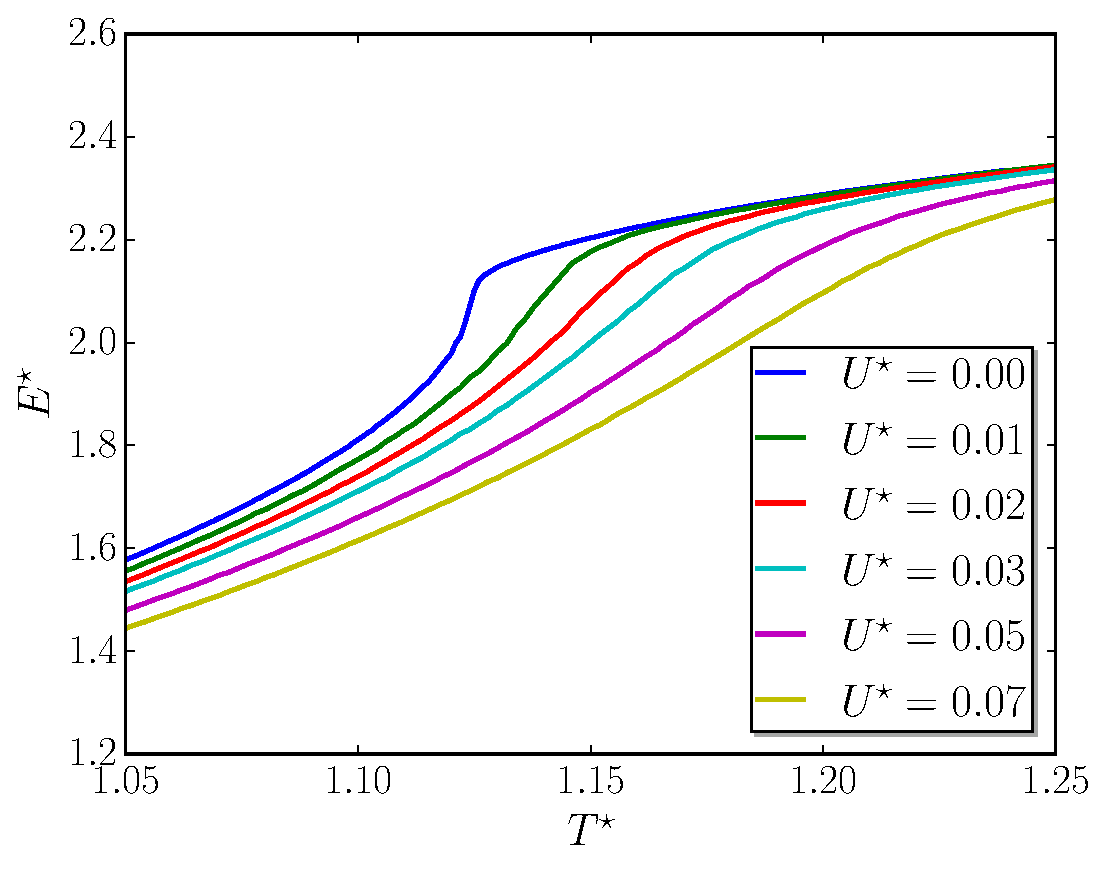
\includegraphics[scale=0.6]{figures/electricField_calo.pdf}
    \caption{Énergie en fonction de la température pour plusieurs champs électriques.}
    	\label{deriveenergie} 
\end{figure}

\newpage
%%%%%%%%%%%%%%%%%%%%%%%%%%%%%%%%%%%%%%%%%%%%%%%%%%%%%%%%%%%%%%%%%%%%%%%%%%%%%%%%%%%%%%%%
%%%%%%%%%%%%%%%%%%%%%%%%%%%%%%%%%%%%%%%%%%%%%%%%%%%%%%%%%%%%%%%%%%%%%%%%%%%%%%%%%%%%%%%%
\section{LCD et transition de Fréedericksz}
%%%%%%%%%%%%%%%%%%%%%%%%%%%%%%%%%%%%%%%%%%%%%%%%%%%%%%%%%%%%%%%%%%%%%%%%%%%%%%%%%%%%%%%%
%%%%%%%%%%%%%%%%%%%%%%%%%%%%%%%%%%%%%%%%%%%%%%%%%%%%%%%%%%%%%%%%%%%%%%%%%%%%%%%%%%%%%%%%

%%%%%%%%%%%%%%%%%%%%%%%%%%%%%%%%%%%%%%%%%%%%%%%%%%%%%%%%%%%%%%%%%%%%%%%%%%%%%%%%%%%%%%%%
%%%%%%%%%%%%%%%%%%%%%%%%%%%%%%%%%%%%%%%%%%%%%%%%%%%%%%%%%%%%%%%%%%%%%%%%%%%%%%%%%%%%%%%%



On a vu que l'application d'un champ électrique faible dans notre modèle de Lebwohl-Lasher avait pour conséquence de modifier la température de transition. Avec ce même modèle, on peut aussi étudier une autre transition: la transition de Fréedericksz qui est utilisée dans les cristaux liquides. 
\medskip

Cette transition se réalise à température constante en faisant varier le champ électrique dans une phase nématique où on ancre les molécules aux bords. On observe alors une compétition entre la contrainte imposée par l'ancrage aux bords qui frustre la phase nématique du système et la contrainte qui tend à aligner les molécules avec le champ électrique. Cette transition présente un intérêt pratique puisque c'est cette dernière qui est utilisée dans les afficheurs à cristaux liquides de type \textit{Twisted nematic}.

\subsection{Fonctionnement d'un écran LCD}

Les écrans à cristaux liquides sont une technologie d'affichage inventée autour de 1970 qui utilise les propriétés polarisantes de deux configuration d'un cristal liquide pour laisser ou non passer la lumière et ainsi afficher des images. 
\medskip

On peut voir sur la Figure \ref{freedericksz} les deux configurations qu'un cristal-liquide adopte dans un afficheur: la première qu'on peut aussi appeler état "allumé" sur la Figure \ref{allume}, et la seconde phase ou état "éteint" sur la Figure \ref{eteint}. Deux filtres polariseurs polarisés selon $y$ et $x$ sont respectivement placés en dessous et au dessus du cristal liquide.



\begin{figure}[h!]
\center
    \begin{subfigure}[b]{0.49\textwidth}
    	\center
        \begin{tikzpicture}
            \node at (0,0) {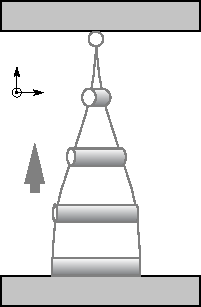
\includegraphics[scale=1.5]{figures/freedericksz_a.pdf}};
            \node at (-2.35,1.25) {$x$}; 
            \node at(-1.2,1.5) {$y$};
            \node at (-2.1,2.4) {$z$};
            \node at (-1.55,0.6) {$\vec{U}^\star$}; 
        \end{tikzpicture} 
    	\caption{Pixel éteint}
    	\label{allume}
    \end{subfigure}	
    \begin{subfigure}[b]{0.49\textwidth}
    	\center
        \begin{tikzpicture}
            \node at (0,0) {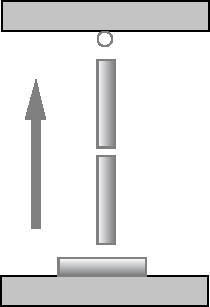
\includegraphics[scale=1.5]{figures/freedericksz_b.pdf}};
            \node at (-1.6,2.2) {$\vec{U}^\star$}; 
        \end{tikzpicture} 
    	\caption{Pixel allumé}
    	\label{etteint}
    \end{subfigure}	
    
    \caption{Schéma de fonctionnement d'un pixel d'un écran LCD \cite{oswald}}
    \label{freedericksz} 
\end{figure}


Dans l'état éteint, le champ électrique est coupé et la seule contrainte exercée sur les molécules est celle causée par l'ancrage aux parois. Cet ancrage a pour conséquence de "tordre" la phase nématique en une hélice ce qui lui permet d'influer sur la polarisation de la lumière qui la traverse. Le cristal liquide tourne la polarisation de 90$\degres$ qui est donc, désormais, orientée selon $\vec{x}$. La lumière peut donc passer le filtre polariseur situé au dessus : le système apparaît transparent.
\medskip

Dans l'état "allumé", on impose un champ électrique fort selon l'axe $z$ ce qui force les molécules à s'aligner dans sa direction. Les molécules alignées ainsi n'ont alors aucune influence sur la polarisation de la lumière les traversant. La lumière incidente n'est pas affectée par le cristal liquide et elle est donc bloquée par le second filtre polariseur : le système apparaît alors opaque.
\medskip

\subsection{Description du modèle}

\subsection{Résultats}

\begin{figure}[h!]
\center
    \begin{subfigure}[b]{0.49\textwidth}
    \centering	    
	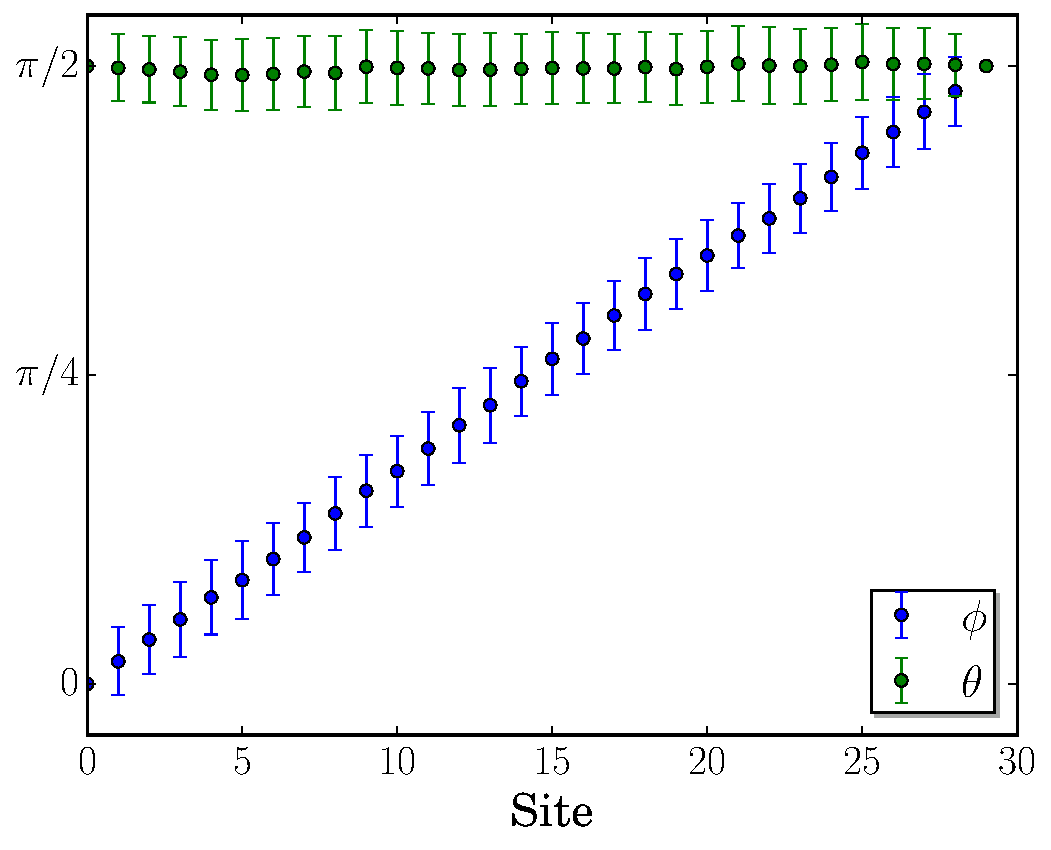
\includegraphics[scale=0.45]{figures/lcd_allume_T01.pdf}
    \caption{temp = 0.1}
    	\label{lcd_allume} 
    \end{subfigure}	
	\begin{subfigure}[b]{0.49\textwidth}
    \centering	    
	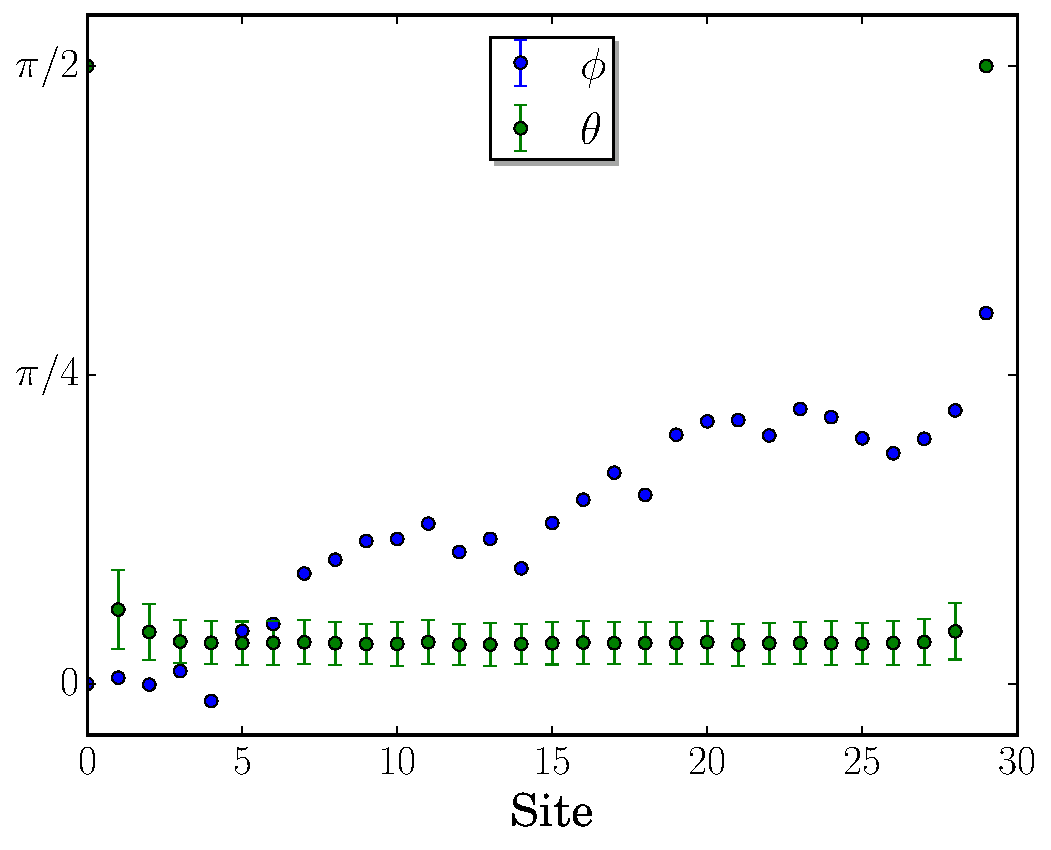
\includegraphics[scale=0.45]{figures/lcd_etteind.pdf}
    \caption{temp = 0.1 elec = 0.5}
    	\label{lcd_etteint} 
    \end{subfigure}

    \caption{yolo}
    \label{lcd}
\end{figure}

TO DO LIST
\begin{itemize}
\item Ecrire les résultats
\item Ecrire la conclusion
\item Ecrire l'abstract
\item Convertir le tout dans le template de merde
\item changer le titre
\item ajouter des références LCD
\item RELIRE TOUT LE RAPPORT
\end{itemize}

\newpage
%%%%%%%%%%%%%%%%%%%%%%%%%%%%%%%%%%%%%%%%%%%%%%%%%%%%%%%%%%%%%%%%%%%%%%%%%%%%%%%%%%%%%%%%
%%%%%%%%%%%%%%%%%%%%%%%%%%%%%%%%%%%%%%%%%%%%%%%%%%%%%%%%%%%%%%%%%%%%%%%%%%%%%%%%%%%%%%%%
\section*{Conclusion}
%%%%%%%%%%%%%%%%%%%%%%%%%%%%%%%%%%%%%%%%%%%%%%%%%%%%%%%%%%%%%%%%%%%%%%%%%%%%%%%%%%%%%%%%
%%%%%%%%%%%%%%%%%%%%%%%%%%%%%%%%%%%%%%%%%%%%%%%%%%%%%%%%%%%%%%%%%%%%%%%%%%%%%%%%%%%%%%%%
\addcontentsline{toc}{section}{Conclusion}


\newpage

\bibliographystyle{unsrt}
\bibliography{biblio} 
\addcontentsline{toc}{section}{Références} 


\end{document}
